%%%%%%%%%%%%%%%%%%%%%%%%%%%
% Inflated Expectations
% Cassandra Grafström and Christopher Gandrud
% 25 November 2013
%%%%%%%%%%%%%%%%%%%%%%%%%%%%

% !Rnw weave = knitr

\documentclass[a4paper]{article}\usepackage[]{graphicx}\usepackage[]{color}
%% maxwidth is the original width if it is less than linewidth
%% otherwise use linewidth (to make sure the graphics do not exceed the margin)
\makeatletter
\def\maxwidth{ %
  \ifdim\Gin@nat@width>\linewidth
    \linewidth
  \else
    \Gin@nat@width
  \fi
}
\makeatother

\definecolor{fgcolor}{rgb}{0.345, 0.345, 0.345}
\newcommand{\hlnum}[1]{\textcolor[rgb]{0.686,0.059,0.569}{#1}}%
\newcommand{\hlstr}[1]{\textcolor[rgb]{0.192,0.494,0.8}{#1}}%
\newcommand{\hlcom}[1]{\textcolor[rgb]{0.678,0.584,0.686}{\textit{#1}}}%
\newcommand{\hlopt}[1]{\textcolor[rgb]{0,0,0}{#1}}%
\newcommand{\hlstd}[1]{\textcolor[rgb]{0.345,0.345,0.345}{#1}}%
\newcommand{\hlkwa}[1]{\textcolor[rgb]{0.161,0.373,0.58}{\textbf{#1}}}%
\newcommand{\hlkwb}[1]{\textcolor[rgb]{0.69,0.353,0.396}{#1}}%
\newcommand{\hlkwc}[1]{\textcolor[rgb]{0.333,0.667,0.333}{#1}}%
\newcommand{\hlkwd}[1]{\textcolor[rgb]{0.737,0.353,0.396}{\textbf{#1}}}%

\usepackage{framed}
\makeatletter
\newenvironment{kframe}{%
 \def\at@end@of@kframe{}%
 \ifinner\ifhmode%
  \def\at@end@of@kframe{\end{minipage}}%
  \begin{minipage}{\columnwidth}%
 \fi\fi%
 \def\FrameCommand##1{\hskip\@totalleftmargin \hskip-\fboxsep
 \colorbox{shadecolor}{##1}\hskip-\fboxsep
     % There is no \\@totalrightmargin, so:
     \hskip-\linewidth \hskip-\@totalleftmargin \hskip\columnwidth}%
 \MakeFramed {\advance\hsize-\width
   \@totalleftmargin\z@ \linewidth\hsize
   \@setminipage}}%
 {\par\unskip\endMakeFramed%
 \at@end@of@kframe}
\makeatother

\definecolor{shadecolor}{rgb}{.97, .97, .97}
\definecolor{messagecolor}{rgb}{0, 0, 0}
\definecolor{warningcolor}{rgb}{1, 0, 1}
\definecolor{errorcolor}{rgb}{1, 0, 0}
\newenvironment{knitrout}{}{} % an empty environment to be redefined in TeX

\usepackage{alltt}
\usepackage{fullpage}
\usepackage[authoryear]{natbib}
\usepackage{setspace}
    \doublespacing
%\usepackage[usenames,dvipsnames]{xcolor}
\usepackage{hyperref}
\hypersetup{
    colorlinks,
    citecolor=black,
    filecolor=black,
    linkcolor=cyan,
    urlcolor=cyan
}
\usepackage{dcolumn}
\usepackage{booktabs}
\usepackage{url}
\usepackage{tikz}
\usepackage{todonotes}
\usepackage[utf8]{inputenc} 
\usepackage{graphicx}

% Set knitr global options



%%%%%%% Title Page %%%%%%%%%%%%%%%%%%%%%%%%%%%%%%%%%%%%%%%%%%%%
\title{Inflated Expectations: How government partisanship shapes monetary policy bureaucrats' inflation forecasts}

\author{Christopher Gandrud \\
                {\emph{Hertie School of Governance}}\footnote{Postdoctoral Researcher. Friedrichstra{\ss}e 180. 10117 Berlin, Germany. Email: \href{mailto:christopher.gandrud@gmail.com}{gandrud@hertie-school.org}. Thank you to the Mark Hallerberg and the Fiscal Governance Centre at the Hertie School of Governance for comments and support. Thank you also to Leonardo Baccini, Vincent Arel-Bundock, Cheryl Schonhardt-Bailey, Tom Stark, and seminar participants at the Hertie School of Governance, London School of Economics, and Yonsei University as well as two anonymous reviewers. This paper was written using {\tt{knitr}} \citep{knitr2013}. It can be entirely replicated from data, analysis source code, and markup files available at: {\url{https://github.com/christophergandrud/GreenBook}}.} \\
                and \\
            Cassandra Grafstr\"{o}m \\
                {\emph{University of Michigan}}\footnote{Ph.D Candidate. 5700 Haven Hall, 505 S. State Street
                Ann Arbor, MI 48109-1045. USA. Email: \href{mailto:cgrafstr@umich.edu}{cgrafstr@umich.edu}.}}
\IfFileExists{upquote.sty}{\usepackage{upquote}}{}

\begin{document}

\maketitle

%%%%%%% Abstract %%%%%%%%%%%%%%%%%%%%%%%%%%%%%%%%%%%%%%%%%%%%
\begin{abstract}

Governments' party identifications can indicate the types of economic policies they are likely to pursue. A common rule of thumb is that left-party governments are expected to pursue policies for lower unemployment, but which may cause inflation. Right-party governments are expected to pursue lower inflation policies. How do these expectations shape the inflation forecasts of monetary policy bureaucrats? If there is a mismatch between the policies bureaucrats \emph{expect} governments to implement and those that they \emph{actually} do, forecasts will be systematically biased. Using US Federal Reserve Staff’s forecasts we test for executive partisan biases. We find that irrespective of actual policy and economic conditions forecasters systematically overestimate future inflation during left-party presidencies and underestimate future inflation during right-party ones. Our findings suggest that partisan heuristics play an important part in monetary policy bureaucrats' inflation expectations.

\end{abstract}

\begin{description}
  \item [{\textbf{Keywords:}}] forecast bias, Federal Reserve bureaucrats, rational partisan cycle, heuristics, inflation, monetary policy
\end{description}

\vspace{0.3cm}


Monetary policy is an inherently forward looking enterprise. Beliefs about the economy's future course significantly guide the setting of interest rates \citep[59]{Goodhart2001}. Government policies have important affects on changes in growth, inflation, and unemployment. Further, a government's party identification can serve as a cue for the types of economic policies that it is likely to pursue during its tenure. A common expectation for the United States is that right-leaning Republicans will pursue policies associated with lower inflation and left-leaning Democrats will pursue policies associated with lower unemployment, but more inflation \cite[see][]{Samuelson1977,HibbsJr1977}. Recent evidence suggests, however, that the real differences in economic policies implemented by the two parties are quite minimal \citep{Bartels2008}. Pursuing monetary policy based on expectations of differences in partisan behavior, as opposed to their general similarities in reality, could lead to systematic mistakes in the setting of monetary policy. It is therefore important to ask how US Federal Reserve Staff incorporate the government's partisan composition when forming expectations of future inflation.

We provide strong evidence that Fed internal inflation forecasts--the forecasts on which monetary policy decisions are based \cite[130]{Adolph2013}--are heavily influenced by an inaccurate presidential partisan rule of thumb or `heuristic'. These forecasts consistently predict that inflation will be lower than it turns out to be under Republican presidencies and that inflation will be higher than it turns out to be under Democratic administrations. Even accounting for changes in monetary policy and a variety of other economic and political factors, Federal Reserve economists over-shoot inflation forecasts for Democrats and under-shoot for Republicans. We find that previous literature on how partisanship may affect monetary policy--primarily work done on partisan preferences \citep{Clark2012,Hakes1988,Sieg1997,Tootell1996} and rational monetary policy expectations \citep{Alesina1987,Alesina1991,Hibbs1994}--is not as useful as a partisan heuristic approach for explaining these predictive failures.

In this paper we first briefly describe bureaucratic inflation forecasting at the US Federal Reserve, why it is important for monetary policy-making, and previous research on sources of bias in it. Academic scholarship on partisanship and Fed forecasting has largely been non-existent. So we introduce the presidential partisan heuristic approach for explaining prediction errors. We also derive major alternative hypotheses about how partisan control of the presidency might shape inflation forecasts by Federal Reserve Staff from the literature on partisanship and monetary policy-making. We then discuss how to measure inflation forecast errors. Using Fed Staff's ``Greenbook'' forecasts we demonstrate that there does appear to be a presidential partisan bias. To understand why these errors exist we test the theories of partisan bias with a series of regression models with data on inflation forecast errors from the 1970s through 2007.\footnote{This is the most complete data set currently available to the public.} Our findings suggest that even when controlling for a number of important economic and political factors, Greenbook forecasts show a distinct presidential partisan bias across presidential terms, not just in the run up to elections, as competing theories would suggest. Rather than being caused by electoral preferences or partisan monetary policy expectations--we find strong evidence supporting our hypothesis that the bias is caused by an incorrect partisan heuristic Fed Staff hold about administrations' likely effect on inflation. Our finding highlights the interaction between political and psychological aspects of how bureaucrats deal with uncertainty that, have previously been ignored by researchers empirically examining monetary policy bureaucracies. In the conclusion we discuss the implications of these findings for monetary policy, election outcomes, and future research directions. 

%%%%%%%%%%%%%% Section 1: Forecasting Inflation at the Fed %%%%%%%%%%%%%%%%%%%%%

\section{Bureaucratic Inflation Forecasting in the United States}

Inflation forecasting is crucial for enabling monetary policy makers to maintain price stability. The primary instrument of monetary policy--interest rates--``only exert their full effect on \ldots inflation with some considerable delay'' \cite[59]{Goodhart2001}. The US Federal Reserve's Greenbook forecasts are an important component of how monetary policy makers' predict future inflation in the United States. Prior to every Federal Open Markets Committee (FOMC) meeting Federal Reserve Staff create a document called the ``Current Economic and Financial Conditions''--Greenbook--that contains information on recent behavior and forecasts of various macroeconomic aggregates assuming no monetary policy change.\footnote{Greenbook data can be found at {\url{http://www.phil.frb.org/research-and-data/real-time-center/greenbook-data/philadelphia-data-set.cfm}} (accessed March 2013). Greenbook forecasts are currently available to the public for each quarter from the fourth quarter of 1965 through the end of 2007. There is a five year lagged release schedule. Also, some forecasts are not available for the entire period.} Federal Reserve Staff make forecasts of various elements of the US and global economies so that the FOMC can make policies appropriate to fulfill the Fed's dual mandate of maintaining maximum employment and price stability.

As \cite{Svensson2005} notes, the accuracy of forecasts is essential to the effectiveness of monetary policy. The FOMC directly uses these forecasts to determine the appropriate monetary policy to pursue and they ``have a large effect on the interest rate chosen by the Fed'' \cite[130]{Adolph2013}. Greenbook forecasts are given to FOMC members one week before each meeting. Staff also present the Greenbook forecasts during FOMC meetings. Expectations, directly influenced by Greenbook forecasts, play a very important part in FOMC decision-making. From FOMC minutes we know that members spend a considerable amount of time discussing prospective economic conditions. In fact much of the FOMC meeting time is used to discuss what economic conditions are likely to be rather than the relative desirability of various outcomes \cite[230]{RomerRomer2008}. Greenbook forecasts directly frame these discussions. What members believe will happen in the future directly influences their policy choices. Higher inflationary expectations increase the likelihood of a member supporting tightening policy in order to slow inflation and an overheating economy; low inflationary expectations increase the likelihood of a preference for loosening monetary policy to bolster growth and employment, all else equal. Therefore, to act as a useful baseline for FOMC decision-making it is important that Greenbook forecasts accurately predict future inflation.

The study of Fed inflation forecasts and their accuracy has been almost exclusively contained within economics with the main concern being the performance of the Fed's forecasts relative to market forecasts \cite[e.g.][]{Romer2000,Faust2007, Gamber2009}. While some studies in the economics literature have examined the biases of particular time periods \cite[e.g.][]{Capistran2006} or bank presidents \cite[e.g.][]{Havrilesky1995}, in our search none considered how government partisanship affects expectations about future inflation at the Federal Reserve.
 
It is important to note that finalized Greenbook forecasts are ``consensus'' forecasts combining \emph{both} econometric models and the professional opinions of forecasters about likely changes in the economy's trajectory not necessarily picked up in these models \citep{Karamouzis1989,Reifschneider1997}. Preferences and/or beliefs about government partisanship, rather than just econometric models based on explicit assumptions, could therefore directly shape Greenbook forecasts.\footnote{Unfortunately, only consensus forecasts are released publicly. It is unfortunately impossible to directly observe the model and judgmental component of the consensus forecasts.} 

The idea that politicians of different partisan stripes might behave differently in office and that their behavior might have different effects on future economic output and inflation is largely uncontroversial for political scientists, especially proponents of rational partisan expectations \cite{Samuelson1977,HibbsJr1977,Alesina1987,Alesina1991,Hibbs1994}.\footnote{See \cite{Franzese2002,Bartels2008} for evidence on the similarities and differences of Democrats and Republicans in office.} However, political scientists have largely not explored whether or how these differences affect Federal Reserve inflation forecasts. The closest attempt made to explore partisan biases in Fed forecasts that we know of was done by \cite{Frendreis2000}. Using simple frequency tables and yearly data, they examined the accuracy of forecasts by the Congressional Budget Office (CBO), presidential administrations', and Federal Reserve Staff. Though they listed the accuracy of Fed inflation forecasts as measured by absolute mean error for the whole period 1979-1997,\footnote{They found that absolute mean errors were similar to the CBO's and less than administrations'.} they \emph{did not examine partisan biases} or any other cause of inaccuracies in Fed forecasts. Their study of partisan biases was entirely confined to a comparison of CBO and administrations' forecasts. 

%%%%%%%%%%%%%%%%%%%%%%%%%%%%% Section 2: Possible Explanations of Fed Inflation Forecast (In)accuracy %%%%%%%%%
\section{Possible Explanations of Fed Inflation Forecast Inaccuracy}

We start to undertake the first significant investigation of possible partisan biases in Fed Staff's inflation forecasting errors in this section by first introducing our presidential partisan heuristic approach. A theory is useful to the extent that it explains a phenomenon better than the most plausible alternatives. So, after introducing partisan heuristics, we posit alternative explanations for the errors that build on previous approaches to understanding the relationship between partisanship and monetary policy decisions that we reformulate for the issue of bureaucratic inflation forecasting.

\subsection{Presidential Partisan Heuristics}

Previous research has shown that (a) central bankers use heuristics or `rules of thumb'--such as Okun's law and the Taylor Rule--to help them understand complex and uncertain economic conditions and (b) that people's economic expectations are shaped by the government's partisan orientation. To understand how presidential partisanship may impact inflation forecasting errors we propose combining these two insights into one coherent approach that we call {\bf{presidential partisan heuristics}}. Let's look at each part of this theory in turn.

\paragraph{Heuristics \& inflation expectations}

We begin with the assumption that Fed Staff have an interest and/or incentive (e.g. because of professional socialization, performance reviews, and regular academic analyses that possibly could provoke FOMC or even Congressional scrutiny) to make the most accurate forecasts possible. This is a reasonable assumption given the numerous studies that have found Fed Staff forecasts to be more accurate than private sector and other government agency forecasts \cite[see][]{Frendreis2000,Romer2000,Gamber2009}.  

However, even if we assume that Fed Staff want to make very accurate predictions and they have access to relatively high quality information, there is still considerable uncertainty about future inflation and the effects of monetary policy on it due to the complexity of economic relationships that create it and the difficulty of adequately observing these relationships \cite[see][22-24]{Schonhardt2013}. In fact \cite{Gamber2009} find that though the overall level of inflation in the United States has decreased since the early 1980s inflation has actually become more difficult to predict as the processes underlying inflation became more unpredictable during the pre-2008/09 period known as the `Great Moderation'. Even if Fed Staff with relatively high quality information want to accurately predict inflation, it is difficult for them to do so. This is precisely the type of situation where we would expect actors to supplement their forecasting models with heuristic judgments in an attempt to create better expectations. Heuristics are intuitions that reduce the complexity associated with making predictions. Considerable psychological and economic research has shown that across a wide range of settings, including among forecasting experts, that people reduce the complexity of predicting uncertain values by using simpler heuristics \citep[see][]{kahneman1973,tverskykahneman1974,Tversky1983,Kahneman2002,kahneman2003}. 

The role of judgment and heuristics to help forecast inflation in light of its complexity has been widely discussed and researched among Federal Reserve staff members themselves. For example, \cite{McNees1990} used individual forecasts to examine situations under which forecasters' judgmental adjustments improved (or didn't) economic forecasts. He found that though judgment can add important information to forecasts, forecasters have a tendency to over adjust their models based on their own judgments. \cite{Orphanides2008} found that FOMC members used a Taylor `rule of thumb' with expected economic conditions when making interest rate decisions. Work by \cite{Tillmann2010Philips} and \cite{KnotekII2007} has found that FOMC members use Phillip's Curve and Okun's Law rules of thumb to predict the relationship between unemployment, inflation, and growth. Overall, the focus in this work has been on rules of thumb based on economic factors.

\paragraph{Partisan inflation expectations}

However, inflation is not a purely economic phenomenon in the sense that government policies beyond monetary policy--narrowly defined as setting interest rates--can affect future inflation. Partisan theories predict that these policies will vary systematically by governments' partisan affinity \citep{Samuelson1977,HibbsJr1977}. One of the main assertions of these partisan theories is that left-leaning Democratic presidents will pursue policies that increase inflation and right-leaning politicians will pursue policies that reduce inflation. [[[CASSIE CAN YOU FILL IN WITH A BREIF STORY?]]] Given this common belief, it would be reasonable to include information about what policies a government is expected to pursue when forecasting inflation.

To our knowledge incorporation of information on government partisanship into monetary bureaucrats inflation expectations has not been examined or explicitly discussed by Fed forecasters. However, previous research has found that members of the public do use presidential partisan heuristics to predict future economic conditions, including inflation. Examining survey data of general assessments of economic health, \cite{Duch2000} found that people perceived both current and future economic conditions differently based on whether or not they shared a partisan affinity with the government. \cite{Snowberg2007} used data from presidential election prediction markets before the 2004 election to examine how partisan expectations move economic indicators. They found that a number of indicators, such as bond yields and exchange rates, moved in directions consistent with standard partisan expectations of policy changes under Democratic and Republican presidents in situations when they thought that candidates from these parties would win.\footnote{Unfortunately, they did not have an economic indicator that could capture changes in inflation expectations.} \cite{Fowler2006} looked specifically at how prediction markets affected futures markets for nominal interest rates. When the probability of a Democrat winning the US Presidency (or Congress) increased, so did interest rate futures. He interprets this finding to suggest that actors expected inflation to increase under a Democratic government. This confirmed a finding using similar methods by \cite{Alesina1997}. \cite{Berlemann2006} extend evidence for a partisan inflation expectations effect to five other developed countries in addition to the United States.

It is important to quickly note that these pieces of research have found evidence that people \emph{expect} economic conditions to be different under different presidents, not that it actually is.

\paragraph{Presidential partisan heuristics \& inflation forecasting errors}

Drawing on these two sets of finding we argue that Fed Staff forecasters are likely to incorporate heuristic about the likely effect of public policies on inflation based on president's party identification. If these expectations do not accurately correspond to actual differences, then we will observe systematic forecasting differences across presidential terms.  

Before discussing why party identification may be used as a heuristic we should consider why we focus on presidents' party identifications. Incorporating information about expected non-monetary policy actions is particularly difficult in the American context. There are many layers of government--national, state, city--that make policies that can impact inflation. Even within the national government there are multiple branches often controlled by different parties that can influence policies. In this case, forecasters may intuitively use a heuristic based on the partisan identification of arguably the single most influential actor in this system--the president--as a way to simplify the complex relationships between politics and inflation. The research discussed in the previous section substantiates this focus by finding that actor's expectations are affected by the president's party identification. 

Presidential partisanship could be used as a ``prototype heuristic'' to help forecasters predict inflation. Prototype heuristics are a general class of heuristic where people substitute the mean or exemplar attribute--prototype--of a category for what they are trying to determine. Prototypes have been found to impact judgments on problems as diverse as the pricing of goods, the effectiveness of painful medical procedures, and the prediction of floods by professional forecasters \cite[]{kahneman2003}. Presidents' partisan identifications are easily observable and available on an intuitive level--i.e. it doesn't require conscious thought to remember them. The probably impact of expected public policies on inflation is not. Fed Staff could use prototypical information about presidential party ID, which is intuitive and readily available, as a substitute for more complete, but more difficult to obtain information about what public policy is likely to be and how it will impact inflation. 

As discussed above, the prototypical Democratic president is been believed to be less concerned with price stability than the prototypical Republican president. The prototypical Republican president therefore pursues policies that dampen inflation and vice versa for the prototypical Democrat. Forecasters using a presidential partisan prototype heuristic would predict inflation to be higher under a Democratic president and lower under a Republican, all else equal. 

Though heuristics can be useful, ``sometimes they lead to severe and systematic errors'' \citep[][1124]{tverskykahneman1974}. In our theory, economists at the Fed have an intuition that Democrats and Republicans behave differently in government and so formulate inflation expectations with this in mind. If this intuition does not accurately correspond to how presidents act, or how their policies impact inflation, forecasts will be systematically biased: overestimates for Democratic presidents, underestimates for Republicans. \cite{Bartels2008} finds evidence that Democratic and Republican presidents do not, in fact, differ significantly in their overall levels of spending, so any expectation that they would pursue policies that would differentially affect inflation in the medium-run would likely be inaccurate.\footnote{\cite{Bartels2008} does not discuss other policies that could affect inflation in the long run, such as changes to labor and financial market regulation. These policies too would be expected to differ by party, however their lags are likely to be quite long and out of the forecasted time frames used in this paper. More specifically, \cite{Franzese2002} finds only moderate evidence for partisan monetary policy differences confined primarily to the period 1973-1982.} These biases should be constant {\emph{throughout a president's term}}. As we will see, this prediction contrasts with the partisan preference and monetary expectation theories, which both assume an intensification of biased behavior as elections approach. Figure \ref{ExpectGraphs} shows an illustrated comparison of the three theories we set out.

It's important to note that in contrast to the typical rational partisan expectations approaches, our model does not require that forecasters be conscious of the heuristic they're using. It can simply work its way subtly into forecasts, particularly in the subjective aspect of the ``consensus forecast" component of the Greenbook. If the models do not conform with other expectations about the economy's current course, based in part on these subtle partisan heuristics, the consensus forecast will be modified accordingly. Further, because this bias would not need to be conscious, the systematic error could easily go unnoticed (as mistakes could occur for any number of idiosyncratic or economic reasons). If the bias goes unnoticed, then it will not be corrected in future inflation predictions.\footnote{This assumption is in contrast to \cite{Grauwe2011}, who assumes that actors actively observe their heuristics and adapt them through trial and error. He does not provide empirical evidence supporting this assumption, however.} This differs from the rational partisan expectations theory \cite[e.g.][]{Alesina1987,Alesina1991,Alesina1997,Hibbs1994}. First, because these beliefs are not updated to account for the lack of partisan differences in spending they are not ``rational". Second, and relatedly, this theory is based on psychological instead of game theoretic reasoning, which allows for the persistence of suboptimal strategies in a way that would be less likely in a rational choice model of this same process given the assumption that the goals of the actors are the same in the two models.





% Define colors for figure
%% See: http://colorbrewer2.org/
\definecolor{DEM}{HTML}{2259B3}
\definecolor{REP}{HTML}{C42B00}

\begin{figure}
  \caption{Stylized Partisan Inflation Forecast Error Predictions}
  \label{ExpectGraphs}
  \begin{center}

    \vspace{0.25cm}

    \tikzstyle{bagMain} = [text width = 5cm]
    \tikzstyle{bagDem} = [text = DEM]
    \tikzstyle{bagRep} = [text = REP]
    
    \tikzstyle{DemLine} = [draw, 
                          color=DEM,
                          opacity=0.9,
                          line width=1.5mm]

    \tikzstyle{RepLine} = [draw, 
                          color=REP,
                          opacity=0.9,
                          line width=1.5mm]

\begin{tikzpicture}

  %%%% Partisan Heuristics
  \node (PP) at (-7, 5) [bagMain]{{\bf{Partisan Heuristics}}};
  \node (E) at (-10.5, 3.25) [bagMain, rotate=90]{{\emph{Forecast Error}}};
  \node (T) at (-7.3, -0.5) [bagMain]{{\emph{Duration of Pres. Term}}};
  
  \draw (-10, 0) -- (-6, 0);
  \draw (-10, 0) -- (-10, 4);


  \draw[DemLine] (-9.5, 3) -- (-6.5, 3); 
  \draw[RepLine] (-9.5, 1) -- (-6.5, 1); 

  \node (R1) at (-6.5, 0.5) [bagRep]{Rep.};
  \node (D1) at (-6.5, 3.5) [bagDem]{Dem.};
  
  %%%% Partisan Preferences
  \node (PP) at (-2, 5) [bagMain]{{\bf{Partisan Preferences}}};
  
  \draw (-5, 0) -- (-1, 0);
  \draw (-5, 0) -- (-5, 4);
  
  \draw[RepLine] (-4.5, 1.9) -- (-2.5, 1.9); 
  \draw[DemLine] (-4.5, 2.1) -- (-2.5, 2.1); 

  \draw[RepLine] (-2.52, 1.9) -- (-1.5, 1); 
  \draw[DemLine] (-2.52, 2.1) -- (-1.5, 3); 


  \node (D2) at (-1.5, 0.5) [bagRep]{Rep.};
  \node (R2) at (-1.5, 3.5) [bagDem]{Dem.};
  
  
  %%%% Monetary Expectations
  
  \node (PP) at (3, 5) [bagMain]{{\bf{Monetary Expectations}}};
  
  \draw (0, 0) -- (4, 0);
  \draw (0, 0) -- (0, 4);

  \draw[RepLine] (0.5, 2.1) -- (2.53, 2.1); 
  \draw[DemLine] (0.5, 1.9) -- (2.53, 1.9); 

  \draw[DemLine] (2.53, 1.9) -- (3.23, 1); 
  \draw[RepLine] (2.53, 2.1) -- (3.23, 3); 

  \node (D3) at (3.5, 3.5) [bagRep]{Rep.};
  \node (R3) at (3.5, 0.5) [bagDem]{Dem.};
  


  \end{tikzpicture}
  \end{center}
\end{figure}




%%%%%%%%%%%%%%%

\subsection{Alternative partisan explanations}

The usefulness of a theory is partially demonstrated by how well it explains events relative to its major competitors. Though no previous studies have examined partisan biases in inflation forecasts, competing theories can be derived from studies that have looked for evidence of partisan preferences manifesting themselves in the FOMC's monetary policy outcomes. Two key strains in this literature have looked for partisan effects as either resulting from a preference for one party over another by members of the FOMC or an expectation that once in office the parties will engage in systematically different policies that will influence inflation, leading the FOMC to support more preferred policies and attempt to inhibit less preferred ones. 

The preference arguments about monetary policy-making assume that a conservative central banker will prefer the election of politicians who hold more similar inflationary preferences (i.e., those with a stronger preference for low inflation) and enact policies to bolster their preferred candidate's prospects of being elected. In the US this would mean that the FOMC would implement policies that supported the electoral prospects of Republican incumbents and harm the electoral prospects of Democratic incumbents \citep{Clark2012,Hakes1988,Sieg1997,Tootell1996}.

Building on this approach, a {\bf{partisan preference theory}} of inflation forecast errors assumes that Fed Staff have a preference for more inflation averse politicians to control the executive and so produce inflation forecasts that would justify the implementation of easy monetary policy under Republican administrations and tight money under Democratic administrations, particularly as presidential elections approach. The FOMC, choosing policy based on these forecasts would then implement monetary policies to optimize its utility function, which would not need to depend upon presidential partisanship at the level of the FOMC.\footnote{It could be that the FOMC either is actually influencing Greenbook forecasts to justify interest rate changes that aid their preferred candidate before elections or that the FOMC and Fed Staff have identical partisan preferences. These would all be observationally equivalent in the absence of detailed case study work. However, as we discuss below, we find no evidence that partisan errors actually change in the run up to elections. As such we do not feel that further case study work on this issue would be useful at this point.} However, because Fed Staffers prefer low inflation to high, they would not necessarily want to produce too loose/tight monetary policy over an entire four year term. Instead, they would want to encourage an economic boost (contraction) near the end of a Republican (Democratic) presidency. This implies that realized inflation would be higher than forecasted during Republican presidencies and lower than forecasted for Democratic presidencies. These effects would be particularly pronounced in the {\emph{quarters running-up to elections}} as Fed Staff attempt to help their favored political party \citep{Beck1987,Grier1987}. Further, accounting for actual changes in monetary policy ought to increase the magnitude of partisan effects. This is because predictions of inflation during Republican presidencies, for example, will be lower than what the staff actually expects. If looser monetary policy is implemented in response to these low inflation forecasts than would have been chosen under the staff's true inflationary expectations, inflation will actually be higher than the staff's true beliefs about inflation under no change in monetary policy.

The rational partisan expectations literature on monetary policy-making assumes that central bankers do not have an innate preference for one party over another, but instead expect Democrats and Republicans to behave differently in office \citep{Alesina1991,Hibbs1994}. It is these behavioral expectations that would lead to different monetary policies under Democratic and Republican presidencies, with the former expected to engage in more expansionary and inflationary policies than the latter. In order to stave off higher inflation under a Democrat the Fed would tighten monetary policy; because Republicans are expected to prefer lower inflation, they will pursue policies in support of that goal and so the FOMC can accommodate Republican presidents' policies without fear of stoking inflation. This argument is again based on the assumed preferences of partisans, but does not require the FOMC to be politically biased as the former does. 

What we call the {\bf{monetary expectations theory}} is based on an assumption of partisan bias in the FOMC rather than among the staff. It assumes that Federal Reserve economists believe members of the FOMC will engage in partisan monetary policy by lowering interest rates under right-leaning administrations and increasing them under left-leaning presidents, as \cite{Clark2012} found, and assumes that the FOMC is doing this to manipulate election outcomes. In this formulation, the Fed Staff has no preference for one party over another, but knows that the FOMC does and so formulates estimates in order to counter the FOMC's policies. If Fed economists believe that the FOMC will choose systematically higher-than-called-for interest rates during Democratic presidencies and vice versa for Republicans, then--assuming they are interested in the implementation of optimal monetary policies--they would produce forecasts that are higher than expected during Republican administrations and lower for Democrats; the {\emph{opposite of what is expected in the partisan preference theory}}. If the FOMC fails to note the compensation made by the Fed Staff, then we would expect that after accounting for implemented policies inflation forecasts would be higher than or equal to realized inflation during Republican terms and lower than or equal to forecasts under Democratic administrations.\footnote{This is illustrated in the center panel of Figure \ref{ExpectGraphs}.} If, however, the FOMC anticipated these compensatory biases in staff forecasts, then the FOMC would discount the Greenbook estimates and continue to implement inflationary policies during Republican administrations and contractionary policies during Democratic ones. If the staff likewise know that they are not being listened to they may randomize their errors, producing an uninformative signal \citep{Crawford1982}. This would result in approximately similar inflation forecast errors for both Republicans and Democrats. However, we largely did not observe this (see below). If the Fed Staff believes that the FOMC will engage in partisan pumping only when presidential elections are approaching, then we would expect no partisan differences in forecasts at the beginning of a presidency but increasing divergence as the term wanes.

The monetary expectations theory models Fed Staff forecasts as partially a function of Staff interactions with the FOMC. What if Greenbook forecasts are even more directly influenced by FOMC members in that members' judgments are directly incorporated in the forecasts? This would have an important substantive implication. All of the partisan theories we have discussed have important policy implications to the extent that they effect FOMC inflation expectations and therefore their interest rate choices. What if this is backward? Why couldn't we assume that it is the FOMC members' partisan biases or preferences that are influencing staff forecasts? 

It is very difficult to empirically determine if and to what extent informal discussions between Fed Staff and FOMC members influence Greenbook forecasts, because these discussion are not observable. However, the formal forecasting process as well as comparisons between Staff and FOMC members' forecasts suggests that the bulk of the influence runs from the Staff to the members rather than the opposite direction.

Greenbook forecasts are presented to FOMC members before FOMC meetings, where expectations are debated at length, and before members make there own biannual formal forecasts.\footnote{Members are required by the 1978 Humphrey-Hawkins Act to make formal forecasts.} If Greenbook forecasts were simply parroting FOMC members' prior expectations then we would expect the two sets of forecasts to be very similar. This has not been the case. \cite{RomerRomer2008} found that FOMC members' forecasts are different from Greenbook forecasts and may in fact be less accurate predictions of inflation. Given that Greenbook forecasts are presented to members directly before FOMC meetings, forecasts act as a reference point from which FOMC members build their own expectations. If attempts by FOMC members to add information to Greenbook forecasts tends to result in less accurate forecasts then it is especially important that the reference point be as accurate as possible.  

\subsection{Forecasting model accuracy}

Finally, before empirically digging into partisan explanations of forecast errors, which would largely be the result of Federal Reserve Staff judgment, it is worth examining the possibility that forecast inaccuracy is the result of \textbf{systematic errors in the staff's predictive econometric models}. Federal Reserve Staff have primarily used two sets of econometric models during the period for which Greenbook data is available.\footnote{This discussion draws heavily on Brayton et al.'s \citeyear{Brayton1997} detailed description of the changes to Federal Reserve forecasting models that took place in 1996.} 

The first simultaneous equation model of the US and world economies were developed and adopted by the Federal Reserve between 1966 and 1975. This model was based on adaptive expectations and largely extrapolated future behavior of the economy from its recent past behavior. New models of the American and world economies' near-term trajectories were introduced in the 1990s, fully replacing the older model in 1996. The Federal Reserve Board US model (FRB/US) and its counterpart for the global economy (FRB/Global) explicitly consider the role of economic expectations in economic behavior. The foundational assumption of adaptive expectations in the old model was replaced with rational or model-consistent expectations. In these models prices are sticky and aggregate demand determines short-run output. Furthermore, monetary policy's effects on the economy are extensively modeled. 

Presumably, the move to rational expectations would improve forecast accuracy relative to the earlier period. The goal of incorporating forward looking actors into the models was to account for an important source of endogeneity in earlier models that could lead to overestimates of important economic indicators under some circumstances and underestimates of those same indicators under others. None of these over or underestimates, however, ought to have been linked to the party of the president. We would, however, expect that the \emph{magnitude} of forecast errors shrank after 1996.\footnote{Unfortunately, we cannot more directly observe model errors. Only the consensus forecasts, i.e. model forecasts combined with judgmental adjustments, are made publicly available.}
 


%%%%%%%%%%%%%%%%%% Section 3: Forecast Accuracy %%%%%%%%%%%%%%%%%%
\section{Federal Reserve Staff's Forecast Accuracy}\label{ForecastAcc}

How accurate are Fed Staff forecasts? We focus on Greenbook forecasts of the GNP/GDP price index forecasts. We choose this indicator of Federal Reserve forecast accuracy because central bankers are believed to be primarily concerned with inflation \citep[e.g.][]{Cukierman1992,Mukherjee2008,Tillmann2008}. It is also the dominant measure of forecast errors used in the economics literature \citep[c.f.][]{Romer2000}. 

We measure accuracy by calculating {\bf{forecast error}} $E$ as the difference between the Greenbook inflation forecast $F$ for a given quarter $q$ and actual inflation $I$ as a proportion of actual inflation:
%
\begin{equation}
    E_{q} = \frac{F_{q} - I_{q}}{I_{q}}.
\end{equation}

This is different from the accuracy measure \cite{Frendreis2000} used in their preliminary examination of forecast errors. They averaged the absolute value of yearly inflation forecast errors over a 19 year period\footnote{i.e. $\frac{|F_{y} - I_{y}|}{19}$} to examine Federal Reserve accuracy. Their measure has a number of drawbacks. First, it does not give us any indication of the direction of the forecast error, which is crucial for examining possible partisan biases. In their comparison of CBO and administrations' forecasts they did use a simple dichotomous directional indicator of accuracy in a given year (i.e. a forecast greater than or less than the actual level). This does not give us a sense of the relative size of the errors and could easily amplify trivial results. Almost any forecast will be above or below the actual inflation level in all but the unusual cases where the forecasts exactly equal the actual inflation level. 

Second, the average of the absolute errors values could be highly skewed by years of unusually large errors, which is more likely in years of higher inflation. This is not a trivial concern because the inflation level varies substantially overtime (see Figure \ref{absolute}).\footnote{\cite{Frendreis2000} also do not include any other indication of the errors' distribution.} So, we choose to focus on proportional rather than absolute errors by quarter to avoid focusing on a parameter that is highly vulnerable to absolute value outliers. Quarterly proportional errors are also more substantively meaningful for comparing errors across time periods.\footnote{Note that the direction and significance of our main findings do not change when we use absolute rather than proportional errors in our estimation models (discussed below). The magnitude does change, but this is to be expected because the range of the absolute inflation errors is much larger than proportional errors. These results are available from the authors upon request.} 

Third, using multi-year or even year-level indicators makes it difficult to examine biases in the run up to an election or any other process that may be observed through variations within years. Using quarterly data--the smallest level available--gives us a much more detailed view of any processes that might influence accuracy.

If the forecasts are unbiased the mean error of the forecasts--using either \cite{Frendreis2000} or our measure--would be indistinguishable from zero. While \cite{Frendreis2000} found that Fed errors were low relative to presidential administrations' on average over a 19 year period and \cite{Romer2000} found that the Fed's internal forecasts  meet this requirement over the full history of Greenbook forecasts, such an amalgamation disguises long periods of over- or under-predicting inflation, as noted in \cite{Capistran2006} and illustrated in Figure \ref{absolute}. Within economics the Fed's forecasts have been examined for evidence of rationality. These studies generally find that the Fed rationally incorporates information into its forecasts, outperforming private forecasts \cite[c.f.][]{Gamber2009}. These studies, however, have rarely incorporated Fed Staff member' political preferences, because Federal Reserve Staffers are assumed to be politically independent.

Our dataset has 169 forecast quarters,\footnote{This is the maximum number of observations. Longer forecasts result in fewer forecasted quarters. Likewise, some forecast lengths are unavailable for the full time period.} spanning the fourth quarter of 1965 through the end of 2007. Greenbook forecasts correspond to those provided for the FOMC meeting closest to the middle of the quarter. We found actual inflation corresponding to each of these quarters\footnote{Inflation was calculated by comparing quarters year-on-year. The exact inflation measure that the Federal Reserve was forecasting changed a number of times, so the measure of actual inflation used to created the forecast error variable changes accordingly. The GNP deflator indicator is used from the beginning of our sample through the end of 1991. From the first quarter of 1992 through the first quarter of 1996 actual inflation is measured with the GDP deflator. From the second quarter of 1996 we use the chain-weighted GDP price index. For more details on how the forecasted quantity changed see the Greenbook data description file available at: \url{http://www.phil.frb.org/research-and-data/real-time-center/greenbook-data/philadelphia-data-set.cfm}. The Greenbook inflation forecast variable we used is called ``PGDPdot''.} using data from the Federal Reserve's FRED website.\footnote{See \url{http://research.stlouisfed.org/fred2/}. Accessed December 2011.} We examine errors made by forecasters in the current quarter and all quarters up to five quarters before.\footnote{The Greenbook contains very incomplete data for forecasts made over longer time spans.} The results are generally the same regardless of the forecast's age, e.g. the results were similar for predictions made $q - 1$ quarters before the forecasted quarter $q$, $q - 2$ quarters before, and so on. In particular the presidential partisan findings are robust regardless of forecast age (see Figure \ref{ExpectValueParty}). For simplicity, the majority of results we show and discuss in detail are from models with forecasts made two quarters beforehand.\footnote{Using these two quarter forecasts restricts our observations because they are rarely available before the 1970s.} Figure \ref{absolute} compares absolute actual inflation for each quarter and inflation forecasts made two quarters before.

%%%%%%%%%%%%%%%%%%%%%%%%%%  Raw Greenbook estimate vs. actual graph
\begin{figure}[t]
    \caption{Greenbook Inflation Forecasts Made 2 Qtr. Beforehand and Actual Quarterly Inflation}
    \label{absolute}
    \begin{center}
    
\begin{knitrout}
\definecolor{shadecolor}{rgb}{0.969, 0.969, 0.969}\color{fgcolor}

{\centering 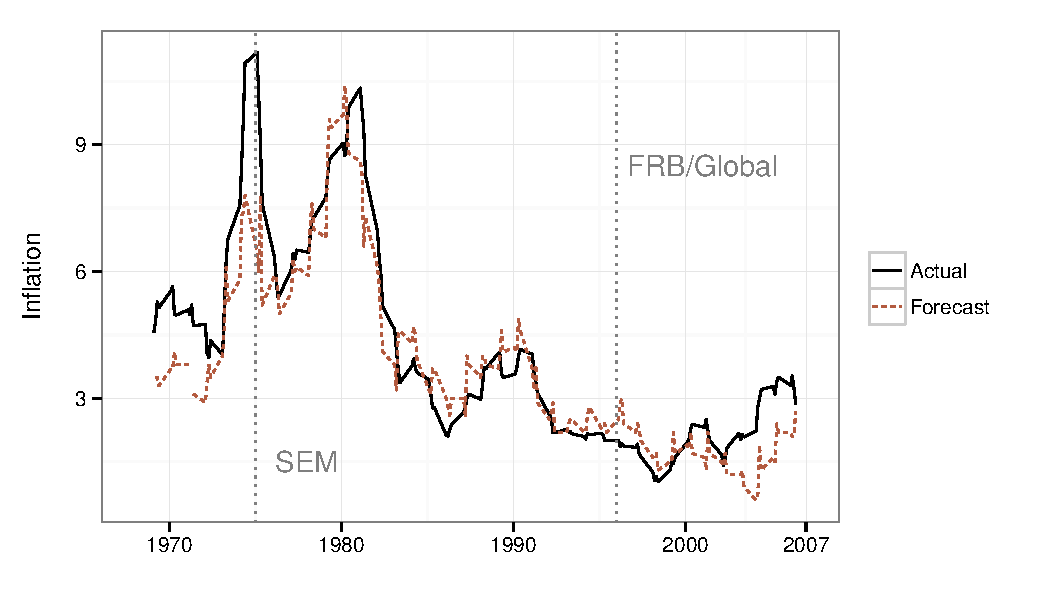
\includegraphics[width=0.8\linewidth]{figure/BaseInflation} 

}



\end{knitrout}

    
    \end{center}
    \begin{singlespace}
        {\scriptsize{The vertical grey dotted line indicates when the Federal Reserve Board Global (FRB/Global) forecasting model was fully implemented.  
                      }}
    \end{singlespace}
\end{figure}


\subsection{Are There Partisan Forecast Errors?}




Unbiased forecasts have a mean error of zero \citep[5]{Bruck2006}. Using this criteria, forecast errors should be the same--ideally with a mean of 0--regardless of the incumbent president's party identification. This is not the case. From the second quarter of 1969\footnote{Data availability for two quarter forecasts before 1969 is lacking.} through 2007 the mean standardized forecast error was -0.04, i.e. forecasters under-predicted inflation by about 4 percent. Our finding of relatively small average error over the entire 35 year period is in line with findings from previous studies. However, the mean errors are noticeably different across Republican compared to Democratic presidencies. Across Republican presidencies it was -11 percent and +13 percent across Democratic presidencies.\footnote{These means are from estimates made two quarters beforehand. Both means are statistically significantly different from 0, the full observation mean, and each other at the 99\% confidence level. For more details see \url{http://bit.ly/WHsRYh}.} On average, inflation was underestimated in Republican presidencies and overestimated in Democratic ones.

Figure \ref{errors_over_time} plots forecast errors across our sample separated by presidential term and party. The first thing to note is that inflation was rarely underestimated during the three Democratic presidential terms in our sample. The underestimates that were made were relatively small. The largest overestimates we see were made during Bill Clinton's (Democratic) presidency. All of the major inflation underestimates were made during Republican presidencies, particularly during Richard Nixon's, Gerald Ford's, and George W. Bush's presidencies. Inflation was often overestimated during the second part of Reagan's first term, his second term, and George H.W. Bush's term. Over this period--often referred to as the Volcker Revolution \citep{Bartels1985}--inflation was suddenly much lower than before (see Figure \ref{absolute}). It may have taken awhile for forecasters to adjust to this new lower level of inflation, particularly because the Fed's own models of the economy assumed that money had no real effects on the economy during this period, even while the FOMC was pursuing aggressive anti-inflation policies.

This summary examination of inflation forecast errors suggests that there may be a presidential partisan bias. Above we posited three different theories of how partisanship might affect inflation forecast errors. In the next section we describe how we go about testing these competing hypotheses.

%%%%%%%%%%%%%%%%%%%%%%%%%%   Greenbook Error Across Time
\begin{figure}[t]
    \caption{Errors in Inflation Forecasts Made 2 Qtr. Beforehand (1969 - 2007)}
    \label{errors_over_time}
    \begin{center}
    
\begin{knitrout}
\definecolor{shadecolor}{rgb}{0.969, 0.969, 0.969}\color{fgcolor}

{\centering \includegraphics[width=0.8\linewidth]{figure/PartisanError} 

}



\end{knitrout}

    
    \end{center}
    \begin{singlespace}
        {\scriptsize{Note: An error of 0 indicates that inflation was perfectly predicted.}}
    \end{singlespace}
\end{figure}



%%%%%%%%%%%%%%%%%% Section 4: Research Methods %%%%%%%%%%%%%%%%%%

\section{Regression Models \& Variables}

We used standard regression models to examine the effects of presidential party ID and elections on the continuous inflation forecast error variable.\footnote{Parametric models are estimated using the \texttt{R} package \texttt{Zelig} \citep{Zelig2012}.} Our main model type was normal linear regression using maximum likelihood estimation of variance.\footnote{In {\tt{Zelig}} this is the {\tt{normal}} model.} To examine if our estimates were dependent on this model type we also ran our analyses with ordinary least squares\footnote{In \texttt{Zelig}, this is the \texttt{ls} model). Because the results were virtually identical, we do not show them below. They are available upon request.} and Bayesian normal linear regression.\footnote{In {\tt{Zelig}} this is the {\tt{normal.bayes}} model.} Bayesian normal linear regression is particularly useful for our relatively small $n$ sample size as it makes ``valid small sample inferences via draws from the exact posterior" \citep[][38]{Zelig2012}.\footnote{Please see \cite{Goodrich2007} for details about Bayesian normal linear regression.} 

As we show below the estimates from all three model types were very similar in direction, magnitude, and statistical significance. They were almost always substantively identical, especially for our key presidential partisan ID variable. 

\subsection{Variables}

In Section \ref{ForecastAcc} we discussed our dependent variable--inflation forecast errors. To examine possible partisan biases we are interested in whether US presidents' partisan identities and/or the existence of an upcoming presidential elections affect these errors. To do this we created {\bf{president party identification}} and {\bf{election period}} variables. The president party ID variable is 1 when the president is a Democrat and 0 when he is a Republican. Since forecast error data is released on a quarterly basis, we consider a president to be sitting from the first quarter after the election.\footnote{Elections are held almost at the midpoint--early November--of an election year's fourth quarter. Presidents are sworn into office near the beginning--20 January--of the following year's first quarter.} We consider quarters to be in the election period either if the presidential election is held in that quarter or in the previous three quarters.\footnote{If $q_{e}$ is a quarter with an election then we code quarters $q_{e}$, $q_{e-1}$, $q_{e-2}$, and $q_{e-3}$ election quarters.} The economic voting literature indicates that it is economic performance in the 6-12 months preceding an American presidential election that seem to matter most for the election's outcome \citep[c.f][]{Gelman1993}. 

To further examine whether or not Federal Reserve Staff were taking into consideration an electoral business cycle either due to a partisan preference or the nearness of an election, we include a variable of the {\bf{quarters until the presidential election}}. This simply counts down from the quarter after the previous election.\footnote{There are 15 quarters before a United States presidential election quarter.} The quarters that included presidential elections are coded as 0. This is used only in models testing for a partisan effect.

The partisan preference and monetary expectations theories both posit that president's party ID and elections have a non-linear interactive relationship with forecast errors. To examine this possibility we include an \textbf{interaction} between the president party ID variable and the square of the quarters until election variable in the analyses.\footnote{An interaction with the non-squared quarters until election variable is also included, following \citep{Brambor2006}.}

United States presidents do not set the level of government expenditure--a major non-monetary policy source of inflation--by themselves. Instead, presidents are constrained by the two houses of Congress. To examine whether or not Federal Reserve Staff are taking into consideration the partisan composition of Congress as well as presidents' party identifications, we include a variable measuring {\bf{Democratic legislators as a proportion of Republican legislators}} in the House of Representatives and a similar variable for the composition of the Senate.\footnote{Data on the number of legislators with Republican and Democratic party IDs was found at infoplease. See {\url{http://www.infoplease.com/ipa/A0774721.html}}. Accessed May 2012.} 

Because each chamber of Congress acts as a veto player on the main fiscal expenditures, any Congressional effect on errors likely works through an \textbf{interaction} between the partisan IDs of Congress and the presidency. There are two types of interaction effects that can be derived from the literature. The first interaction possibility is that Federal Reserve Staff, using simple rational partisan expectations, presume that a Democratic president would be able to get policies closer to their ideal point when there is a Congress with similar preferences. If a Democratic president faced chambers of Congress controlled by Democrats, presumably Federal Reserve Staff would expect even higher fiscal expenditures and therefore even higher inflation. Conversely, Republican presidents with a Republican-controlled Congress may be even better at cutting spending, leading to even lower inflation.\footnote{The inflationary effect of these policies may be mitigated if they were offset by higher or lower taxes respectively.}

The second possibility is based largely on Krause's \citeyearpar{Krause2000} work on the effect of partisan divisions on fiscal deficits in the United States. He finds partisan fragmentation can play a role in increasing federal deficits. Higher political conflict, he argues, ``results in equilibrium fiscal outcomes that favor greater spending and/or a willingness to lower taxes since politicians will exhibit a greater proclivity in providing voters with program benefits and to delay its payment" \citep[][542]{Krause2000}. Because of this Federal Reserve Staff may anticipate higher government borrowing when the presidency and houses of Congress are controlled by different parties. We are therefore agnostic about the theoretical direction of this interaction.

If prediction errors are largely the result of systematically biased economic forecasting models we would expect errors to change when the models changed. In particular, we would expect a decrease in the magnitude of errors around 1996 when the Federal Reserve Board's new US and Global Behavioral Equation Models were introduced. To examine this we include a {\bf{FRB/Global Model}} dummy variable. It equals one for all quarters from the first quarter of 1996 onward. It is zero otherwise.

Greenbook forecasts are based on the assumption that monetary policy will not change between when the prediction is made and the time period it is predicting.\footnote{While the Fed Staff also produce forecasts under alternative monetary policies in the so-called ``Bluebook," these data are not available in a readily usable format (i.e., not in a dataset but only in the original reports themselves) and thus are not used in the forecasting error literature.} However, since these forecasts are used in the setting of interest rates, this assumption often does not hold and forecast errors may occur if monetary policy changes in the interim. If this is the case monetary policy changes would have a negative relationship with forecast errors. When the FOMC raises interest rates inflation may decline, causing the original forecast to have been too high and vice versa. To control for monetary policy changes we include a variable of {\bf{standardized changes to the discount rate}} from the quarter the Greenbook prediction was made to the quarter it is predicting.\footnote{We averaged the discount rate over each quarter. Then we used the average discount rate $D$ in each quarter $q$ to create the variable $\Delta D_{q}$ using the simple formula: $\Delta D_{q} = \frac{D_{q} - D_{q-2}}{D_{q}}$. Note that the Federal Reserve changed how it used the discount rate and referred it at the beginning of 2003. To address this issue we primarily used data on the United States' discount rate recorded by the International Monetary Fund. Their data only goes back to the fourth quarter of 1982. So, before that we use the Federal Reserve's measure of the discount rate. Both of these variables are found in the FRED database at the St. Louis Federal Reserve (accessed July 2012). } The discount rate is one of the Federal Reserve's main tools for influencing the interest rate, especially the Fed Funds rate.\footnote{A similar {\bf{relative changes in the Fed Funds rate}} variable was included in some preliminary analyses. However, it did not change the results substantially and was estimated to have a similar effect on errors as the discount rate variable.}

We included a number of variables to examine if Federal Reserve inflation forecast errors are affected by incorrect assumptions about how levels of government expenditure impact inflation. These variables are the percentage of {\bf{current government expenditure to GDP}}, {\bf{government debt to GDP}},\footnote{Results for debt to GDP are not shown because it was never statistically significant in any of the models.} and \textbf{deficit to GDP}. Expenditure and debt are on a quarterly basis, while federal deficits are measured annually.\footnote{All three of these variables are from the FRED database, accessed October 2012 and January 2013.}

To examine how broader economic factors may be related to forecast errors we include variables of the {\bf{GDP output gap}}, {\bf{unemployment rate}} and {\bf{recession}}. The GDP output gap is the potential GDP as a percentage of real GDP. It is in nominal terms. The recession variable is a dummy for whether or not the United States was in a recession.\footnote{All three of these variables are from the FRED database, accessed June and October 2012.} 

Finally, we include a series of dummies for the sitting {\bf{Federal Reserve Board Chair}}.\footnote{Chairs for the years in our analysis are William McChesney Martin, Jr., Arthur Burns, G. William Miller, Paul Volcker, Alan Greenspan, and Ben Bernanke.} Further variables used to examine additional omitted variable bias are discussed in the paper's Supplementary Materials.

\section{Results}

In this section we graphically present results from a number of regression model specifications and discuss our findings. Full coefficient estimate lists can be found in tables \ref{OutputNL} and \ref{OutputNB}. There is little difference between the coefficients estimated using normal linear and Bayesian linear regression models (see Figure \ref{CoefComparePlots}).\footnote{In all of the Bayesian regressions we use the {\tt{Zelig}} default 1,000 MCMC burn-in iterations and 10,000 iterations after burn-in. We use the Heidelberger-Welch diagnostic to examine whether or not the Markov Chains converged to their stationary distributions.} As the ordinary least squares estimates were essentially identical to the normal linear regression estimates, we do not show them here.

We remove quarters from the sample where forecasters would not have known who the president would be because the president had not yet been elected for that quarter. For models where the dependent variable is forecasts made two quarters beforehand this means removing the first two quarters of each presidential term.\footnote{In this case 19 quarters are removed.} Results from these restricted data sets are fairly similar to those from the full data set.




\begin{figure}[t]
    \caption{95\% Confidence Bands for Coefficients from a Multiple Parametric Model Specifications}
    \label{CoefComparePlots}
    \begin{center}

\begin{knitrout}
\definecolor{shadecolor}{rgb}{0.969, 0.969, 0.969}\color{fgcolor}

{\centering 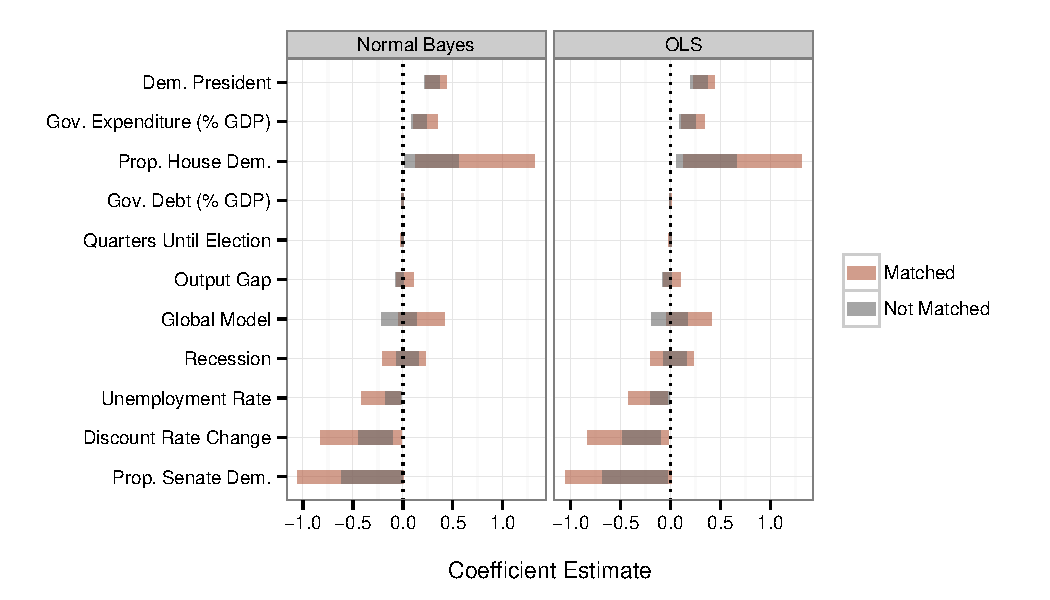
\includegraphics[width=0.95\linewidth]{figure/CoefComparePlots} 

}



\end{knitrout}

    \end{center}
    \begin{singlespace}
        {\scriptsize{Please see the full estimates tables in tables \ref{OutputNL} and \ref{OutputNB}.}}
    \end{singlespace}
\end{figure}

\paragraph{Presidential Party Identification}

Our main finding is that Democratic party identification had a strong positive association with Federal Reserve Staff inflation forecast errors. Inflation forecast errors are estimated to be higher during Democratic presidencies than Republican ones even when we control for the numerous economic and political variables discussed earlier. This finding is robust across virtually all model specifications. Notably, the estimated effect holds even when we control for actual government expenditure and government deficits. This suggests that Federal Reserve Staff are not simply incorrectly predicting spending--which may be correlated with presidential party ID--and its effect on inflation. Instead, they either additionally have a partisan preference or are using partisan heuristics.\footnote{Note that the direction of the relationship--forecasts being overestimated during Democratic presidencies--is the opposite of that predicted by the Monetary Expectations theory.} We can further narrow down the likely causes of the bias by looking at an interaction between presidential party ID and election timing. The estimated presidential party ID effect remains constant across presidential terms, even as the election nears. This finding is what we would expect if Federal Reserve Staff have a presidential partisan heuristic, but not a partisan preference or an expectation that FOMC policy will change as elections near.


\begin{figure}[t]
    \caption{Simulated Expected Inflation Forecast Error for Republican and Democratic Presidencies}
    \label{ExpectValueParty}
    \begin{center}

%%% Code is only run when there are changes, since it is very computationally intensive.
\begin{knitrout}
\definecolor{shadecolor}{rgb}{0.969, 0.969, 0.969}\color{fgcolor}

{\centering 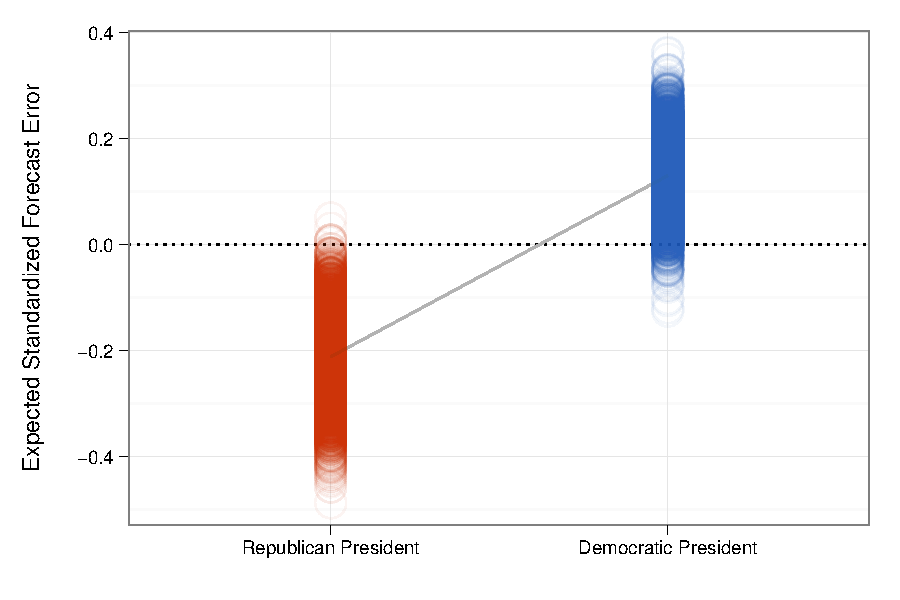
\includegraphics[width=0.81\linewidth]{figure/ExpectValueParty} 

}



\end{knitrout}





    \end{center}
    \begin{singlespace}
        {\scriptsize{Simulated from a normal linear regression. Variables included are generally the same as those in Model A6 from Table \ref{OutputNL}. The discount rate change variable is adjusted to reflect the change in the discount rate from the quarter when the forecast was made. Discount rate change was not included for the model predicting forecasts made in the present quarter since it is always 0. \\ Each model excludes every quarter when the forecasters would not have known who the president was. Because of this, the number of observations used in each model is noted on the figure. \\ The figure shows 950 simulations per presidential party ID type. They are the middle 95\% of 1000 simulations per presidential party ID type. The grey lines connect the groups' means.}}
    \end{singlespace}
\end{figure}

Following \cite{King2000}, we simulated expected standardized forecast errors for Democratic and Republican presidencies, holding the other covariates at their means, to get a sense of approximately how big the presidential partisan bias is when using different forecast lags. Results from these simulations are shown in Figure \ref{ExpectValueParty}.\footnote{Figure \ref{ExpectValueParty}. The graph uses visually-weighted regression techniques to communicate uncertainty \citep[see][]{Hsiang2012,Gandrud2013visual}.} There is some variation in the predicted error magnitude depending on how many quarters ago the forecast was made. Nonetheless it is notable that inflation is always predicted to be higher than it really is in Democratic presidencies and lower than it is in Republican presidencies.

For forecasts made two quarters in advance, we expect that the Fed overestimates inflation by 20 percent during Democratic presidencies, all else equal. We expect the average inflation error during Republican presidencies to be approximately -12 percent. Given that the first quantile of the inflation errors is -22 and the third is 13, \emph{these estimates indicate that partisan biases are on average a large contributor to the overall magnitude of inflation forecasting errors}. These results hold up even when we rerun the models on data where we dropped individual presidential terms (see Table \ref{OutputNLPresDrop}) and Fed chairman terms.\footnote{These are available from the authors upon request.} This indicates that the results are not being driven by one outlier presidential or chairman term.

Clearly, at least from the 1970s through 2007, Fed Staff were overly pessimistic about Democratic presidents' effect on inflation and overly optimistic about Republican presidents' effect. 

\paragraph{Presidential Elections}

Do Federal Reserve Staff also take into consideration election timing as the partisan preference and monetary expectations theories predict? 

We do not find much, if any, evidence that inflation forecast errors were associated with elections either independent of presidential party ID or in interaction with it. Estimates of the relationship between the quarters until election variable and forecast errors\footnote{This variable is obviously omitted from the models with the election period variable because they are highly correlated.} also fails to provide any evidence that inflation errors are related to elections. 

We examined the monetary policy and partisan preference theories of forecast errors with an interaction between the president's party ID variable and the square of the time to election variable. We used the square of the time to election variable to try to capture the non-linear predicted effect of elections on errors made by the monetary and partisan preference theories (see left-hand and center panels of Figure \ref{ExpectGraphs}). However, when we include the interactions coefficient on the president's party ID variable is robust whereas neither the election variables nor the interaction terms are statistically significant. This is also true when we use the non-squared version of the time to election variable (please see the Supplementary Material). Thus we do not find evidence for either the partisan preference or monetary expectations theories.

Fed Staff do not appear to be over-estimating inflation when a Democratic president is running for re-election in an attempt to influence the FOMC to raise interest rates and lower the president's chances of winning as hypothesized in the partisan preference theory prediction. These findings have clear implications for how we understand the potential causes of Greenbook partisan inflation forecast biases as well as FOMC interest rate decisions around elections. It seems that FOMC \emph{members}, not their staff, are driving the increases in the Fed Funds Rate around elections when Democrats are in power that \cite{Clark2012} observe. Interestingly, staff also do not seem to compensate for FOMC partisan biases in an attempt to moderate FOMC-driven partisan electoral business cycles. Thus, we find no evidence in favor of the monetary expectations theory.

%%%%%%% President/Congress Interaction Plot %%%%%%%%
\begin{figure}[t]
    \caption{Simulated Expected Inflation Forecast Error with Interactions Between President Party ID and Congressional Party Control (Qtr. 2 forecasts)}
    \label{InterPlot}
    \begin{center}

\begin{knitrout}
\definecolor{shadecolor}{rgb}{0.969, 0.969, 0.969}\color{fgcolor}

{\centering 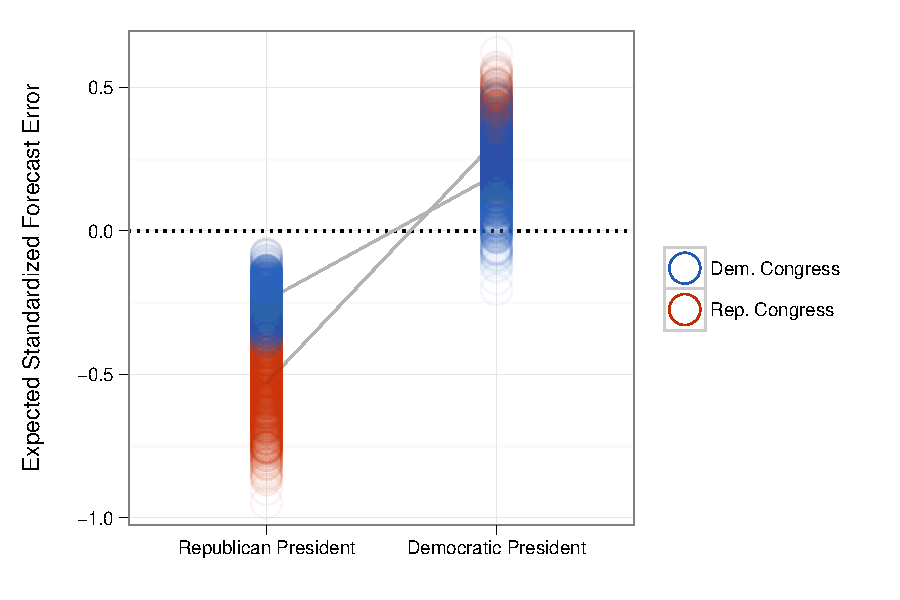
\includegraphics[width=0.7\linewidth]{figure/InterPlot} 

}



\end{knitrout}


    \end{center}
    \begin{singlespace}
        {\scriptsize{Simulated from normal linear regressions. Expected errors in the left-side graph are from Model A9 in Table \ref{OutputNL} and the right-side estimates are from Model A13 from Table \ref{OutputPL}. The figure shows 950 simulations per fitted value. They are the middle 95\% of 1000 simulations per fitted value. The gray lines connect the groups' means.  \\ Both the House and Senate Democratic/Republican variables were set at 1.2 for Democratic congresses and 0.8 for Republican congresses.}}
    \end{singlespace}
\end{figure}

\paragraph{Partisan Control of Congress}

Might Federal Reserve Staff be taking into consideration not only the president's party identification, but also the partisan composition of Congress?  We estimate parametric models with two-way and three-way interactions between presidential and congressional party identification to look for evidence in favor of either of the two ways we identified that presidential and congressional partisan ID might be related to forecast errors. All of the partisan interactions are generally statistically significant. To make substantive sense of these estimated interactions we again generate simulations to find expected inflation forecast errors at various levels of the presidential and congressional party identification variables. Figure \ref{InterPlot} shows simulation results with highly contrasting fitted variable values: one party control of the executive and both legislative bodies compared to a situation where one party controls the presidency and the other controls both houses of Congress.\footnote{Both the House and Senate Democratic/Republican variables are set at 1.2 for Democratic congresses and 0.8 for Republican congresses.} 

The first thing we should notice in Figure \ref{InterPlot} is how presidential partisan identification still seems to be driving the direction of the inflation forecast errors: inflation is underestimated during Republican presidencies and overestimated during Democratic ones, regardless of what party controls Congress. The substantive effect of congressional control on forecast errors is in the magnitude of the over- or underestimates. In particular, Republican control of Congress seems to exacerbate the differences already noted between Democratic and Republican executives. Inflation is very underestimated for Republican presidencies with Republican congresses and more overestimated for Democratic presidents facing an opposition controlled legislature. There may be an expectation among Fed Staff that solidly Republican governments will cut expenditure much more than they actually do. Forecast errors are also slightly higher on average with Democratic presidencies and Republican congresses compared to when both are controlled by Democrats. This finding would fit with a story where Fed Staff believe spending will be higher with a divided government. 

Despite some evidence for an interaction between congressional and presidential party identification, it is not clear at this time how these results can be consistently explained across Democratic and Republican presidencies. 

%%%%%%% Table of non-matched data with normal linear parametric model %%%%%%%%

\begin{table}[ht]
    \caption{Normal Linear Regression Estimation of Covariate Effects on 2 Qtr. Inflation Forecast Error}
    \label{OutputNL}
    \vspace{0.25cm}
    \begin{center}
    \scalebox{0.9}{
    {\tiny
 
\begin{tabular}{ l D{.}{.}{1}D{.}{.}{1}D{.}{.}{1}D{.}{.}{1}D{.}{.}{1}D{.}{.}{1}D{.}{.}{1}D{.}{.}{1}D{.}{.}{1}D{.}{.}{1}D{.}{.}{1}D{.}{.}{1}D{.}{.}{1}D{.}{.}{1} } 
\hline 
  & \multicolumn{ 1 }{ c }{ A1 } & \multicolumn{ 1 }{ c }{ A2 } & \multicolumn{ 1 }{ c }{ A3 } & \multicolumn{ 1 }{ c }{ A4 } & \multicolumn{ 1 }{ c }{ A5 } & \multicolumn{ 1 }{ c }{ A6 } & \multicolumn{ 1 }{ c }{ A7 } & \multicolumn{ 1 }{ c }{ A8 } & \multicolumn{ 1 }{ c }{ A9 } & \multicolumn{ 1 }{ c }{ A10 } & \multicolumn{ 1 }{ c }{ A11 } & \multicolumn{ 1 }{ c }{ A12 } & \multicolumn{ 1 }{ c }{ A13 } & \multicolumn{ 1 }{ c }{ A14 } \\ \hline
 %                    & A1              & A2              & A3              & A4              & A5              & A6              & A7              & A8              & A9              & A10             & A11             & A12             & A13             & A14            \\ 
Intercept            & 3.5 ^\dagger   & 3.6 ^\dagger   & 3.6 ^\dagger   & 4.9 ^{**}       & 4.3 ^*          & 4.1 ^*          & 2.1             & 2.1             & 1.3             & 2.0             & 3.9 ^*          & 3.3 ^\dagger   & 3.4 ^\dagger   & -1.8 ^{***}    \\ 
                     & (2.0)           & (2.1)           & (2.1)           & (1.7)           & (2.0)           & (1.7)           & (2.0)           & (2.0)           & (2.2)           & (2.1)           & (1.8)           & (1.8)           & (1.8)           & (0.4)          \\ 
Recession            & 0.0             & 0.0             & 0.0             & 0.1 ^\dagger   & 0.0             & 0.1             & 0.1             & 0.1             & 0.0             & 0.0             & 0.1 ^*          & 0.1 ^\dagger   & 0.1             &                \\ 
                     & (0.1)           & (0.1)           & (0.1)           & (0.1)           & (0.1)           & (0.1)           & (0.1)           & (0.1)           & (0.1)           & (0.1)           & (0.0)           & (0.0)           & (0.1)           &                \\ 
Expenditure/GDP      & 0.1 ^{***}      & 0.1 ^{***}      & 0.1 ^{***}      & 0.2 ^{***}      &                 & 0.2 ^{***}      & 0.2 ^{***}      & 0.2 ^{***}      & 0.1 ^{***}      & 0.2 ^{***}      & 0.1 ^{***}      & 0.2 ^{***}      & 0.1 ^{***}      &                \\ 
                     & (0.0)           & (0.0)           & (0.0)           & (0.0)           &                 & (0.0)           & (0.0)           & (0.0)           & (0.0)           & (0.0)           & (0.0)           & (0.0)           & (0.0)           &                \\ 
Output Gap           & -0.1 ^{**}      & -0.1 ^{**}      & -0.1 ^{**}      & -0.1 ^{***}     & -0.0 ^*         & -0.1 ^{***}     & -0.1 ^*         & -0.1 ^*         & -0.0            & -0.1 ^*         & -0.1 ^{***}     & -0.1 ^{***}     & -0.1 ^{***}     &                \\ 
                     & (0.0)           & (0.0)           & (0.0)           & (0.0)           & (0.0)           & (0.0)           & (0.0)           & (0.0)           & (0.0)           & (0.0)           & (0.0)           & (0.0)           & (0.0)           &                \\ 
Discount Rate Change & -0.1            & -0.1            & -0.1            & -0.2 ^*         & -0.3 ^*         & -0.3 ^{**}      & -0.3 ^{**}      & -0.3 ^{**}      & -0.3 ^{**}      & -0.3 ^{**}      & -0.2 ^*         & -0.2 ^*         & -0.2 ^*         &                \\ 
                     & (0.1)           & (0.1)           & (0.1)           & (0.1)           & (0.1)           & (0.1)           & (0.1)           & (0.1)           & (0.1)           & (0.1)           & (0.1)           & (0.1)           & (0.1)           &                \\ 
Unemployment Rate    & -0.0            & -0.0            & -0.0            & 0.0             & 0.0             & 0.0             & -0.1            & -0.1            & -0.1            & -0.1            & -0.0            & -0.0            & 0.0             &                \\ 
                     & (0.0)           & (0.0)           & (0.0)           & (0.0)           & (0.0)           & (0.0)           & (0.0)           & (0.0)           & (0.0)           & (0.0)           & (0.0)           & (0.0)           & (0.0)           &                \\ 
Qtr. to Election     &                 & 0.0             &                 &                 &                 & 0.0             & 0.0             & 0.0             & -0.0            & 0.0             & 0.0 ^*          & 0.0 ^*          & 0.0 ^*          &                \\ 
                     &                 & (0.0)           &                 &                 &                 & (0.0)           & (0.0)           & (0.0)           & (0.0)           & (0.0)           & (0.0)           & (0.0)           & (0.0)           &                \\ 
Qrt. to Election2    &                 & -0.0            &                 &                 &                 &                 &                 &                 & 0.0             &                 &                 &                 &                 &                \\ 
                     &                 & (0.0)           &                 &                 &                 &                 &                 &                 & (0.0)           &                 &                 &                 &                 &                \\ 
Election Period      &                 &                 & -0.0            &                 &                 &                 &                 &                 &                 &                 &                 &                 &                 &                \\ 
                     &                 &                 & (0.0)           &                 &                 &                 &                 &                 &                 &                 &                 &                 &                 &                \\ 
Pres. Party ID       &                 &                 &                 & 0.3 ^{***}      & 0.4 ^{***}      & 0.3 ^{***}      & 0.3 ^{***}      & 0.3 ^{***}      & 0.3 ^*          & 0.3 ^{***}      & 1.0 ^{***}      & 1.1 ^{***}      & 1.7 ^*          & 2.1 ^{**}      \\ 
                     &                 &                 &                 & (0.0)           & (0.1)           & (0.0)           & (0.0)           & (0.0)           & (0.1)           & (0.0)           & (0.1)           & (0.2)           & (0.7)           & (0.8)          \\ 
Deficit/GDP          &                 &                 &                 &                 & -0.1 ^{**}      &                 &                 &                 &                 &                 &                 &                 &                 &                \\ 
                     &                 &                 &                 &                 & (0.0)           &                 &                 &                 &                 &                 &                 &                 &                 &                \\ 
FRB/GlobalModel      &                 &                 &                 &                 &                 & 0.1 ^\dagger   &                 &                 & 0.1             &                 &                 &                 &                 &                \\ 
                     &                 &                 &                 &                 &                 & (0.0)           &                 &                 & (0.1)           &                 &                 &                 &                 &                \\ 
Senate Dem/Rep       &                 &                 &                 &                 &                 &                 & -0.3 ^\dagger  & -0.3 ^\dagger  & -0.3 ^*         &                 & -0.2            & -0.1            & 0.6             & 0.8 ^*         \\ 
                     &                 &                 &                 &                 &                 &                 & (0.1)           & (0.1)           & (0.2)           &                 & (0.1)           & (0.1)           & (0.4)           & (0.3)          \\ 
House Dem/Rep        &                 &                 &                 &                 &                 &                 & 0.3 ^*          & 0.3 ^*          & 0.3 ^*          &                 & 0.5 ^{***}      & 0.4 ^{**}       & 1.1 ^{***}      & 1.6 ^{***}     \\ 
                     &                 &                 &                 &                 &                 &                 & (0.1)           & (0.1)           & (0.1)           &                 & (0.1)           & (0.1)           & (0.3)           & (0.3)          \\ 
Pres*Qrt. Election   &                 &                 &                 &                 &                 &                 &                 &                 & 0.0             &                 &                 &                 &                 &                \\ 
                     &                 &                 &                 &                 &                 &                 &                 &                 & (0.0)           &                 &                 &                 &                 &                \\ 
Pres*Qrt. Election2  &                 &                 &                 &                 &                 &                 &                 &                 & -0.0            &                 &                 &                 &                 &                \\ 
                     &                 &                 &                 &                 &                 &                 &                 &                 & (0.0)           &                 &                 &                 &                 &                \\ 
Burns                &                 &                 &                 &                 &                 &                 &                 &                 &                 & 0.3 ^{***}      &                 &                 &                 &                \\ 
                     &                 &                 &                 &                 &                 &                 &                 &                 &                 & (0.1)           &                 &                 &                 &                \\ 
Greenspan            &                 &                 &                 &                 &                 &                 &                 &                 &                 & 0.2 ^*          &                 &                 &                 &                \\ 
                     &                 &                 &                 &                 &                 &                 &                 &                 &                 & (0.1)           &                 &                 &                 &                \\ 
Martin               &                 &                 &                 &                 &                 &                 &                 &                 &                 & 0.2             &                 &                 &                 &                \\ 
                     &                 &                 &                 &                 &                 &                 &                 &                 &                 & (0.1)           &                 &                 &                 &                \\ 
Miller               &                 &                 &                 &                 &                 &                 &                 &                 &                 & 0.3 ^\dagger   &                 &                 &                 &                \\ 
                     &                 &                 &                 &                 &                 &                 &                 &                 &                 & (0.1)           &                 &                 &                 &                \\ 
Volcker              &                 &                 &                 &                 &                 &                 &                 &                 &                 & 0.3 ^{**}       &                 &                 &                 &                \\ 
                     &                 &                 &                 &                 &                 &                 &                 &                 &                 & (0.1)           &                 &                 &                 &                \\ 
Pres*House           &                 &                 &                 &                 &                 &                 &                 &                 &                 &                 & -0.5 ^{***}     &                 & -1.4            & -2.4 ^{**}     \\ 
                     &                 &                 &                 &                 &                 &                 &                 &                 &                 &                 & (0.1)           &                 & (0.8)           & (0.9)          \\ 
Pres*Senate          &                 &                 &                 &                 &                 &                 &                 &                 &                 &                 &                 & -0.7 ^{***}     & -0.2            & -0.1           \\ 
                     &                 &                 &                 &                 &                 &                 &                 &                 &                 &                 &                 & (0.1)           & (0.8)           & (0.7)          \\ 
House*Senate         &                 &                 &                 &                 &                 &                 &                 &                 &                 &                 &                 &                 & -0.5 ^*         & -0.9 ^{***}    \\ 
                     &                 &                 &                 &                 &                 &                 &                 &                 &                 &                 &                 &                 & (0.2)           & (0.2)          \\ 
Pres*House*Senate    &                 &                 &                 &                 &                 &                 &                 &                 &                 &                 &                 &                 & 0.5             & 0.9 ^\dagger  \\ 
                     &                 &                 &                 &                 &                 &                 &                 &                 &                 &                 &                 &                 & (0.5)           & (0.5)           \\
 $N$                  & 135             & 135             & 135             & 135             & 135             & 135             & 135             & 135             & 135             & 135             & 135             & 135             & 135             & 135            \\ 
AIC                  & -4.1            & -0.3            & -2.2            & -54.6           & -7.7            & -54.9           & -56.0           & -56.0           & -52.4           & -57.7           & -83.3           & -80.1           & -85.0           & -49.7          \\ 
BIC                  & 65.6            & 92.6            & 79.2            & 26.7            & 73.6            & 49.7            & 60.2            & 60.2            & 110.3           & 93.4            & 44.5            & 47.7            & 77.7            & 43.3           \\ 
$\log L$            & 26.1            & 32.2            & 29.1            & 55.3            & 31.9            & 63.4            & 68.0            & 68.0            & 82.2            & 80.8            & 85.7            & 84.1            & 98.5            & 56.8            \\ \hline
 \multicolumn{15}{l}{\footnotesize{Standard errors in parentheses}}\\
\multicolumn{15}{l}{\footnotesize{$^\dagger$ significant at $p<.10$; $^* p<.05$; $^{**} p<.01$; $^{***} p<.001$}} 
\end{tabular} 


    }
    }
    \end{center}
\end{table}

%%%%%%% Table of pres_party matched data with Bayesian normal linear parametric 
% latex table generated in R 3.0.2 by xtable 1.7-1 package
% Mon Nov 25 15:35:08 2013
\begin{table}[ht]
\centering
\caption{Bayesian Normal Linear Regression Estimation of Covariate Effects on 2 Qtr. Inflation Forecast Error} 
\label{OutputNB}
{\small
\begin{tabular}{lccccc}
  \hline
Variables & Mean & SD & 2.5\% & 50\% & 97.5\% \\ 
  \hline
Intercept & 3.62 & 1.56 & 0.54 & 3.63 & 6.73 \\ 
  Pres. Party ID & 0.30 & 0.04 & 0.23 & 0.30 & 0.37 \\ 
  Recession & 0.06 & 0.05 & -0.05 & 0.06 & 0.16 \\ 
  Qtr. to Election & -0.00 & 0.00 & -0.01 & -0.00 & 0.00 \\ 
  Expenditure/GDP & 0.15 & 0.02 & 0.11 & 0.15 & 0.18 \\ 
  Output Gap & -0.07 & 0.02 & -0.10 & -0.07 & -0.03 \\ 
  Discount Rate Change & -0.26 & 0.09 & -0.43 & -0.26 & -0.09 \\ 
  Unemployment Rate & -0.01 & 0.03 & -0.06 & -0.01 & 0.05 \\ 
  Global Model & 0.10 & 0.04 & 0.02 & 0.10 & 0.18 \\ 
  sigma2 & 0.04 & 0.00 & 0.03 & 0.04 & 0.04 \\ 
   \hline
\end{tabular}
}
\end{table}




%%%%%%% Table of non-matched data with Normal Linear Regression parametric model Dropping presidential terms %%%%%%%%

\begin{table}[ht]
    \caption{Normal Linear Regression Estimation of Covariate Effects on 2 Qtr. Inflation Forecast Error, Dropping Presidential Terms}
    \label{OutputNLPresDrop}
    \vspace{0.25cm}
    \begin{center}
    \scalebox{0.9}{
    {\tiny
 
\begin{tabular}{ l D{.}{.}{1}D{.}{.}{1}D{.}{.}{1}D{.}{.}{1}D{.}{.}{1}D{.}{.}{1}D{.}{.}{1}D{.}{.}{1}D{.}{.}{1}D{.}{.}{1}D{.}{.}{1} } 
\hline 
  & \multicolumn{ 1 }{ c }{ Nixon 1 } & \multicolumn{ 1 }{ c }{ Nixon 2 } & \multicolumn{ 1 }{ c }{ Ford } & \multicolumn{ 1 }{ c }{ Carter } & \multicolumn{ 1 }{ c }{ Reagan 1 } & \multicolumn{ 1 }{ c }{ Reagan 2 } & \multicolumn{ 1 }{ c }{ GHW Bush } & \multicolumn{ 1 }{ c }{ Clinton 1 } & \multicolumn{ 1 }{ c }{ Clinton 2 } & \multicolumn{ 1 }{ c }{ GW Bush 1 } & \multicolumn{ 1 }{ c }{ GW Bush 2 } \\ \hline
 %                    & Nixon 1         & Nixon 2         & Ford            & Carter          & Reagan 1        & Reagan 2        & GHW Bush        & Clinton 1       & Clinton 2       & GW Bush 1       & GW Bush 2      \\ 
Intercept            & 3.9 ^\dagger   & 4.3 ^*          & 4.0 ^*          & 6.2 ^{**}       & 4.2 ^*          & 3.0             & 3.8 ^*          & 2.6             & 4.4 ^{**}       & 4.6 ^{**}       & 3.7 ^*         \\ 
                     & (2.1)           & (1.8)           & (1.7)           & (2.0)           & (1.8)           & (1.9)           & (1.9)           & (2.0)           & (1.6)           & (1.6)           & (1.7)          \\ 
Recession            & 0.0             & 0.1             & 0.1             & 0.0             & 0.1             & 0.1             & 0.0             & 0.0             & 0.1             & 0.1             & 0.0            \\ 
                     & (0.1)           & (0.1)           & (0.1)           & (0.1)           & (0.1)           & (0.1)           & (0.1)           & (0.1)           & (0.1)           & (0.1)           & (0.1)          \\ 
Expenditure/GDP      & 0.2 ^{***}      & 0.2 ^{***}      & 0.2 ^{***}      & 0.1 ^{***}      & 0.2 ^{***}      & 0.1 ^{***}      & 0.2 ^{***}      & 0.2 ^{***}      & 0.2 ^{***}      & 0.1 ^{***}      & 0.2 ^{***}     \\ 
                     & (0.0)           & (0.0)           & (0.0)           & (0.0)           & (0.0)           & (0.0)           & (0.0)           & (0.0)           & (0.0)           & (0.0)           & (0.0)          \\ 
Output Gap           & -0.1 ^{**}      & -0.1 ^{***}     & -0.1 ^{***}     & -0.1 ^{***}     & -0.1 ^{***}     & -0.1 ^{**}      & -0.1 ^{***}     & -0.1 ^{**}      & -0.1 ^{***}     & -0.1 ^{***}     & -0.1 ^{***}    \\ 
                     & (0.0)           & (0.0)           & (0.0)           & (0.0)           & (0.0)           & (0.0)           & (0.0)           & (0.0)           & (0.0)           & (0.0)           & (0.0)          \\ 
Discount Rate Change & -0.3 ^{**}      & -0.3 ^{**}      & -0.3 ^{**}      & -0.3 ^{**}      & -0.3 ^{**}      & -0.3 ^{**}      & -0.3 ^{**}      & -0.3 ^{**}      & -0.3 ^{**}      & -0.2 ^\dagger  & -0.2 ^\dagger \\ 
                     & (0.1)           & (0.1)           & (0.1)           & (0.1)           & (0.1)           & (0.1)           & (0.1)           & (0.1)           & (0.1)           & (0.1)           & (0.1)          \\ 
Unemployment Rate    & -0.0            & 0.0             & -0.0            & 0.1             & -0.0            & -0.0            & 0.0             & -0.0            & 0.0             & 0.0             & -0.0           \\ 
                     & (0.0)           & (0.0)           & (0.0)           & (0.0)           & (0.0)           & (0.0)           & (0.0)           & (0.0)           & (0.0)           & (0.0)           & (0.0)          \\ 
Qtr. to Election     & 0.0             & -0.0            & 0.0             & 0.0             & 0.0             & 0.0             & -0.0            & 0.0             & -0.0            & -0.0            & 0.0            \\ 
                     & (0.0)           & (0.0)           & (0.0)           & (0.0)           & (0.0)           & (0.0)           & (0.0)           & (0.0)           & (0.0)           & (0.0)           & (0.0)          \\ 
Pres. Party ID       & 0.3 ^{***}      & 0.3 ^{***}      & 0.3 ^{***}      & 0.4 ^{***}      & 0.3 ^{***}      & 0.3 ^{***}      & 0.3 ^{***}      & 0.3 ^{***}      & 0.2 ^{***}      & 0.3 ^{***}      & 0.3 ^{***}     \\ 
                     & (0.0)           & (0.0)           & (0.0)           & (0.0)           & (0.0)           & (0.0)           & (0.0)           & (0.0)           & (0.0)           & (0.0)           & (0.0)          \\ 
FRB/GlobalModel      & 0.1             & 0.1 ^\dagger   & 0.1 ^\dagger   & 0.1 ^*          & 0.1 ^\dagger   & 0.1             & 0.1 ^\dagger   & 0.2 ^{**}       & 0.1 ^{**}       & 0.0             & 0.0            \\ 
                     & (0.1)           & (0.0)           & (0.0)           & (0.0)           & (0.0)           & (0.0)           & (0.0)           & (0.0)           & (0.0)           & (0.0)           & (0.1)           \\
 $N$                  & 123             & 129             & 126             & 121             & 121             & 121             & 121             & 121             & 121             & 121             & 125            \\ 
AIC                  & -40.5           & -48.9           & -51.1           & -45.7           & -49.7           & -44.0           & -38.6           & -54.4           & -67.2           & -71.9           & -50.0          \\ 
BIC                  & 60.7            & 54.0            & 51.0            & 55.0            & 50.9            & 56.6            & 62.0            & 46.3            & 33.5            & 28.8            & 51.9           \\ 
$\log L$            & 56.3            & 60.5            & 61.5            & 58.8            & 60.9            & 58.0            & 55.3            & 63.2            & 69.6            & 71.9            & 61.0            \\ \hline
 \multicolumn{12}{l}{\footnotesize{Standard errors in parentheses}}\\
\multicolumn{12}{l}{\footnotesize{$^\dagger$ significant at $p<.10$; $^* p<.05$; $^{**} p<.01$; $^{***} p<.001$}} 
\end{tabular} 


    }
    }
    \end{center}
\end{table}

\paragraph{Government Expenditure}

It seems that Federal Reserve Staff may also overestimate the effect of government expenditure on inflation. This is indicated by a consistently positive and significant coefficient for the government expenditure variable, even when controlling for president's party ID. Perhaps this is because Fed Staff not only have a presidential partisan heuristic, but also a similar government expenditure heuristic where expenditure is believed to have a larger impact on inflation than it really does. It is plausible that the mechanism for this could be either an informal heuristic that affects the judgemental part of the forecasts or an incorrect assumption built into the formal forecasting models.

\paragraph{Deficits} We avoided including deficits and federal expenditures in the same models, because they are fairly highly correlated.\footnote{In models where they were both included (not shown, but available upon request) the deficit variable's estimated coefficient was very unstable and regularly switched sign.} Deficits as a proportion of GDP had a negative relationship with inflation forecast errors. This is in the same direction as our finding for government expenditure, because a positive deficit to GDP value indicates a surplus, i.e. less spending relative to revenue. Note that this estimate was not robust across all models.

\paragraph{FRB Global Forecasting Model}

The introduction of the FRB/Global behavioral equation forecasting model in 1996 does not seem to have begun a new era of reduced inflation forecasting error. In one model specification the estimate was statistical significance at the 10 percent level. However it was not robust across most model specifications. This suggests that forecasts made after the introduction of this approach were not more accurate than those made before it. 

\paragraph{Changes to the Discount Rate}

As expected, relative changes to the discount rate are often found to be negatively associated with inflation forecast errors. Increasing the discount rate could result in lower inflation than expected and vice versa. Controlling for FOMC policy does not change the estimated relationship between presidential party ID and errors. It should be noted that the discount rate results are not robust across all of the models\footnote{See in particular results from models using matched data in the Supplementary Materials.} 

\paragraph{Further Robustness Checks}

The Supplementary Material's section of the paper includes further robustness checks that we used to test the strength of our key findings. In particular we explore other specifications of the president party ID and time to election interaction, the key variable's relationships with an orthoganal variable--unemployment forecast errors--the inclusion of economic and political shocks, such as oil price and labor productivity changes as well as armed conflicts, as well as parametric models with pre-analysis data matched on presidential party ID and election period. Please see the Supplementary Materials for more information. 

\section*{Discussion: Partisanship \& bureaucratic inflation forecast errors}

Do Fed inflation forecasts have a partisan bias? According to the evidence from our research: yes. Federal Reserve Staff seem to have systematically overestimated inflation during Democratic presidencies and underestimated it during Republican ones for at least a 38 year period between 1969 and the end of 2007. This finding is robust across numerous model specifications where a variety of economic, bureaucratic, and other political factors were controlled for. 

In the course of our research we also found that Fed Staff tend to overestimate the inflationary effect of government spending and perhaps deficits independent of the partisanship bias. Conceptually, the bias nonetheless runs in the same direction as the presidential partisanship bias. More spending, which Democrats are often expected to prefer, is anticipated to increase inflation more than it actually does.\footnote{Of course Fed Staff could be incorrectly forecasting government expenditure and deficits. This could then somehow contribute to biased inflation forecasts. However, we do not have access to complete Fed estimates of government expenditure and deficits to test this possibility.} It is unlikely that Greenbook forecasting models explicitly incorporate the president's party identification, so we can be reasonably certain that the partisan bias enters as a heuristic in the judgmental side of the forecasting process. Predicted inflationary effects for government spending could very well be incorporated into the formal forecasting models. So, the government expenditure bias that we found could be either the result of incorrect explicit model assumptions or heuristics.

Interestingly, in light of recent research on FOMC policy-making, we found no relationship between inflation forecast errors and elections either independent of presidential party identification or in interaction with it. This suggests that any relationship between monetary policy decisions and US presidential election timing is neither the result of partisan preferences that Fed Staff members may have, nor beliefs that Fed Staff may hold about the FOMC's presidential election preferences. 

Given the consistency of the bias across presidents' terms, it appears that Fed Staff's partisan inflation forecast bias may be the result of a partisan heuristic. Like heuristics generally, the partisan heuristic may help Fed Staffers simplify very complex phenomenon, with the negative side effect that it creates systematic prediction errors. These errors may not have been noticed by staffers because, so far, few if anyone has been looking for them. Indeed, the only piece of research we found examining Fed forecasting errors and partisan forecasting biases \cite[i.e.][]{Frendreis2000} did not actually look for partisan biases in Fed forecasts. We find that inflation forecasts are consistently underestimated when Republicans hold the White House and are consistently overestimated during Democratic administrations. This is a new finding that helps us better understand how monetary policy bureaucrats address uncertainty and complexity in the relationship between policy and the economy. Though heuristic rules of thumb have been researched extensively in the economics literature \citep[e.g.][]{kahneman1973, tverskykahneman1974, kahneman2003} and various economically-based monetary policy rules of thumb have been discussed by academic researchers and monetary policy makers themselves \cite[e.g.][]{McNees1990,Orphanides2008}, the possibility of political heuristics impacting monetary policy bureaucrats’ expectations has previously been ignored. It also challenges previous assumptions in the literature \cite[see in particular][]{Grauwe2011} that actors adapt their heuristics and expectations based on new information. Hopefully our findings will give forecasters an impetus to do just that so that they can more accurately forecast inflation.

What has been the monetary policy and electoral impact of Federal Reserve Staff partisan bias? Our research so far cannot definitively answer this, but it does motivate future research and point in a clear direction. It may be that higher inflation forecasts during Democratic presidencies spur the FOMC to raise interest rates and dampen the money supply generally. The opposite could happen during Republican presidencies. If this is the case, the economy would be inadvertently stimulated during Republican presidencies and depressed during Democratic ones, with electoral implications. The economic voting literature has repeatedly found that poor economic performance results in less electoral support for incumbent presidents \citep[e.g.][]{Alvarez1998, Bloom1975, LewisBeck1988, Powell1993}. Thus, if these partisan biases in inflation forecasts are leading to more restrictive monetary policy during Democratic presidencies and more expansive monetary policy during Republican presidencies, the economic voting mechanism may run afoul of important normative concerns about democratic accountability. Determining the extent to which these biases are shaping monetary policy is therefore an important next step in understanding the linkage between Fed inflation forecasts and larger questions of democracy. This is a very important issue that needs further investigation.

%%%%%%% References %%%%%%%%%%%%

\clearpage

\bibliographystyle{apsr}
\bibliography{GreenBook.bib}


%%%%%% Supplementary Material %%%%%%%%%%
\clearpage

\section*{Supplementary Material for:\\ \emph{Inflated Expectations: How government partisanship shapes monetary policy bureaucrats' inflation forecasts}}

In this Supplementary Material section we present further robustness checks to further test the strength of our main empirical findings.  

\subsection*{Mid-term election timing}

To further check the robustness of the possible effect of elections on errors we examined models with election variables that included mid-term elections--non-presidential elections when the House of Representatives and a portion of the Senate is elected--in addition to presidential elections. As before, we subsetted the data to exclude quarters when the forecasters would not have know who the winners of the elections would be. This variable was, like the equivalent variable that only included presidential election timing, statistically insignificant. Its interaction with presidential party ID was also insignificant. Table \ref{MidTerm} shows results from two of these models.

\begin{table}[ht]
    \caption{Normal Linear Regression Estimation with Standardized 2 Qrt. Inflation Forecasting Error as the Dependent Variable and a Quarter to Election Variables that Included Midterms (non-matched data set)}
    \label{MidTerm}
    \vspace{0.25cm}
    \begin{center}
    {\small{
 
\begin{tabular}{ l D{.}{.}{1}D{.}{.}{1} } 
\hline 
  & \multicolumn{ 1 }{ c }{ SM1 } & \multicolumn{ 1 }{ c }{ SM2 } \\ \hline
 %                                & SM1             & SM2            \\ 
Intercept                        & -0.2            & -0.2           \\ 
                                 & (2.2)           & (2.2)          \\ 
Recession                        & 0.0             & 0.0            \\ 
                                 & (0.1)           & (0.1)          \\ 
Expenditure/GDP                  & 0.1 ^{***}      & 0.1 ^{***}     \\ 
                                 & (0.0)           & (0.0)          \\ 
Output Gap                       & -0.0            & -0.0           \\ 
                                 & (0.0)           & (0.0)          \\ 
Discount Rate Change             & -0.3 ^{**}      & -0.3 ^{**}     \\ 
                                 & (0.1)           & (0.1)          \\ 
Unemployment Rate                & -0.1 ^\dagger  & -0.1 ^\dagger \\ 
                                 & (0.0)           & (0.0)          \\ 
Pres. Party ID                   & 0.3 ^{***}      & 0.3 ^{***}     \\ 
                                 & (0.0)           & (0.1)          \\ 
Qrt. Midterm/Pres. Election      & 0.0             & 0.0            \\ 
                                 & (0.0)           & (0.0)          \\ 
FRB/GlobalModel                  & 0.1             & 0.1            \\ 
                                 & (0.1)           & (0.1)          \\ 
Senate Dem/Rep                   & -0.4 ^*         & -0.4 ^*        \\ 
                                 & (0.2)           & (0.2)          \\ 
House Dem/Rep                    & 0.4 ^*          & 0.4 ^*         \\ 
                                 & (0.2)           & (0.2)          \\ 
Pres*Qrt. Midterm/Pres. Election &                 & 0.0            \\ 
                                 &                 & (0.0)           \\
 $N$                              & 115             & 115            \\ 
AIC                              & -39.0           & -37.0          \\ 
BIC                              & 81.8            & 94.8           \\ 
$\log L$                        & 63.5            & 66.5            \\ \hline
 \multicolumn{3}{l}{\footnotesize{Standard errors in parentheses}}\\
\multicolumn{3}{l}{\footnotesize{$^\dagger$ significant at $p<.10$; $^* p<.05$; $^{**} p<.01$; $^{***} p<.001$}} 
\end{tabular} 


    }}
    \end{center}
\end{table}

\subsection*{President party ID and election timing linear interaction}

In the body of the paper we presented results from models with president party ID and the square of quarters to the election. The first model in table \ref{SupTable1} shows results with an interaction between president party ID and the non-squared linear version of election timing. The results are substantively equivalent to those with the squared version. In both cases the interaction is not statistically significant.

\subsection*{Economic and violent conflict shocks}

We examined if economic or violent conflict shocks may impact inflation forecast errors. First we examined if the underlying level of inflation could impact the standardized forecast errors. Perhaps if price changes are very volatile, e.g. inflation is very high, then there may be larger errors. We examined this possibility by including two absolute inflation variables in the models: (a) the \textbf{absolute inflation level in the quarter being forecasted} for and (b) \textbf{absolute inflation in the quarter prior} to when the forecast was made.\footnote{In Table \ref{SupTable1} this is referred to as `Lag 3 Abs. Inflation'.} The second and third models in Table \ref{SupTable1} show that including these variables did not substantively change the presidential partisan ID results. Absolute inflation in the quarter being forecasted for has a statistically significant negative relationship with forecast errors. Referring back to Figure \ref{errors_over_time} in the main paper, this makes empirical sense as periods of high inflation in the 1970s were actually times when the standardized forecast error was relatively small. This finding persists even if we use absolute inflation forecast errors (i.e. $F_{q} - I_{q}$) as the dependent variable. This can be seen in Model S10 in Table \ref{SupTable2}.

Second, we consider other economic and political shocks. Perhaps oil price shocks, for example in the late 1970s, increased inflation forecast errors. To examine this possibility we gathered data from the FRED database\footnote{Accessed October 2013.} on the \textbf{change in the West Texas Crude price} from the quarter in the previous year. Similarly, maybe labor productivity increases, especially in the 1990s created unexpected economic conditions and therefore inflation forecasting errors. To examine this possibility we gathered data from the United States Bureau of Labor Statistics on non-farm business \textbf{labor productivity}.\footnote{The series ID was PR85006092. Accessed October 2013.} The variable is in terms of the percent change from the previous quarter at the annual rate. Finally, perhaps violent conflict also created unexpected economic conditions. To examine this we created an indicator of the \textbf{total number of armed conflicts per year} using data from Uppsala Conflict Data Program/Peace Research Institute Oslo \citep{Harbom2012,Gleditsch2002}. 

As we see in tables \ref{SupTable1} and \ref{SupTable2} the productivity changes and the number of armed conflicts were not robustly associated with inflation forecasting errors. Oil price changes were found to be statistically significantly associated with errors. This association was negative so that high price increases are related to lower errors. This mirrors our finding for the absolute inflation level. High absolute inflation and high oil price increases are associated in time during our observation period. They were both particularly high during the mid to late 1970s. This was simultaneously a period of relatively small inflation forecast errors. 

This finding initially seems counter-intuitive. We might expect that inflation forecasting is easier when there is less inflation, lower oil price volatility, and so on. However, recent economic research has shown that inflation in the United States has became more difficult to forecast from the 1990s as the reduction in inflation variability has been largely due to a reduction in the `predictable component' of inflation \citep[see][]{Gamber2009}. 

Notably, the presidential partisan ID variable's effect does not change in magnitude, direction, or statistical significance when any of the shock variables are included. It also doesn't change when we use our standardized measure or inflation forecasting errors or absolute errors.

\begin{table}[ht]
    \caption{Normal Linear Regression Estimation with Standardized 2 Qtr. Inflation Forecasting Error as the Dependent Variable and Additional Independent Variables (non-matched data set)}
    \label{SupTable1}
    \vspace{0.25cm}
    \begin{center}
    {\tiny{
 
\begin{tabular}{ l D{.}{.}{1}D{.}{.}{1}D{.}{.}{1}D{.}{.}{1}D{.}{.}{1}D{.}{.}{1}D{.}{.}{1} } 
\hline 
  & \multicolumn{ 1 }{ c }{ S1 } & \multicolumn{ 1 }{ c }{ S2 } & \multicolumn{ 1 }{ c }{ S3 } & \multicolumn{ 1 }{ c }{ S4 } & \multicolumn{ 1 }{ c }{ S5 } & \multicolumn{ 1 }{ c }{ S6 } & \multicolumn{ 1 }{ c }{ S7 } \\ \hline
 %                    & S1              & S2              & S3              & S4              & S5              & S6              & S7             \\ 
Intercept            & 2.0             & 2.3             & 1.3             & 2.3             & 2.2             & 2.3             & 2.5            \\ 
                     & (2.0)           & (1.9)           & (2.1)           & (1.9)           & (2.0)           & (2.0)           & (2.0)          \\ 
Recession            & 0.0             & 0.1 ^*          & 0.1             & 0.1             & 0.0             & 0.0             & 0.1            \\ 
                     & (0.1)           & (0.1)           & (0.1)           & (0.1)           & (0.1)           & (0.1)           & (0.1)          \\ 
Expenditure/GDP      & 0.1 ^{***}      & 0.1 ^{***}      & 0.1 ^{***}      & 0.1 ^{***}      & 0.1 ^{**}       & 0.1 ^{***}      & 0.1 ^{**}      \\ 
                     & (0.0)           & (0.0)           & (0.0)           & (0.0)           & (0.0)           & (0.0)           & (0.0)          \\ 
Output Gap           & -0.0 ^*         & -0.0 ^*         & -0.0            & -0.0 ^*         & -0.0 ^*         & -0.0 ^*         & -0.0 ^*        \\ 
                     & (0.0)           & (0.0)           & (0.0)           & (0.0)           & (0.0)           & (0.0)           & (0.0)          \\ 
Discount Rate Change & -0.3 ^{**}      & -0.2 ^\dagger  & -0.3 ^{**}      & -0.2 ^*         & -0.3 ^{**}      & -0.3 ^{**}      & -0.2 ^\dagger \\ 
                     & (0.1)           & (0.1)           & (0.1)           & (0.1)           & (0.1)           & (0.1)           & (0.1)          \\ 
Unemployment Rate    & -0.1            & -0.0            & -0.1            & -0.1            & -0.1            & -0.1            & -0.0           \\ 
                     & (0.0)           & (0.0)           & (0.0)           & (0.0)           & (0.0)           & (0.0)           & (0.0)          \\ 
Pres. Party ID       & 0.3 ^{***}      & 0.3 ^{***}      & 0.3 ^{***}      & 0.3 ^{***}      & 0.3 ^{***}      & 0.3 ^{***}      & 0.3 ^{***}     \\ 
                     & (0.1)           & (0.0)           & (0.0)           & (0.0)           & (0.0)           & (0.0)           & (0.0)          \\ 
Qtr. to Election     & 0.0             & 0.0             & 0.0             & -0.0            & 0.0             & 0.0             & -0.0           \\ 
                     & (0.0)           & (0.0)           & (0.0)           & (0.0)           & (0.0)           & (0.0)           & (0.0)          \\ 
FRB/GlobalModel      & 0.1             & 0.1 ^*          & 0.1 ^\dagger   & 0.1             & 0.1 ^\dagger   & 0.1             & 0.1            \\ 
                     & (0.1)           & (0.1)           & (0.1)           & (0.1)           & (0.1)           & (0.1)           & (0.1)          \\ 
Senate Dem/Rep       & -0.3 ^*         & -0.3 ^*         & -0.4 ^*         & -0.3 ^*         & -0.3 ^*         & -0.4 ^*         & -0.3 ^\dagger \\ 
                     & (0.2)           & (0.1)           & (0.2)           & (0.1)           & (0.2)           & (0.2)           & (0.2)          \\ 
House Dem/Rep        & 0.3 ^*          & 0.4 ^{**}       & 0.3 ^*          & 0.3 ^*          & 0.3 ^\dagger   & 0.3 ^*          & 0.3 ^\dagger  \\ 
                     & (0.1)           & (0.1)           & (0.1)           & (0.1)           & (0.1)           & (0.1)           & (0.1)          \\ 
Pres*Qrt. Election   & -0.0            &                 &                 &                 &                 &                 &                \\ 
                     & (0.0)           &                 &                 &                 &                 &                 &                \\ 
Abs Inflation        &                 & -0.0 ^{**}      &                 &                 &                 &                 &                \\ 
                     &                 & (0.0)           &                 &                 &                 &                 &                \\ 
Lag 3 Abs. Inflation &                 &                 & -0.0            &                 &                 &                 &                \\ 
                     &                 &                 & (0.0)           &                 &                 &                 &                \\ 
Oil Price Change     &                 &                 &                 & -0.0 ^\dagger  &                 &                 & -0.0 ^\dagger \\ 
                     &                 &                 &                 & (0.0)           &                 &                 & (0.0)          \\ 
Productivity Change  &                 &                 &                 &                 & 0.0             &                 & 0.0            \\ 
                     &                 &                 &                 &                 & (0.0)           &                 & (0.0)          \\ 
No. Armed Conflicts  &                 &                 &                 &                 &                 & -0.0            & -0.0           \\ 
                     &                 &                 &                 &                 &                 & (0.0)           & (0.0)           \\
 $N$                  & 135             & 135             & 132             & 135             & 135             & 135             & 135            \\ 
AIC                  & -55.3           & -64.8           & -52.2           & -59.0           & -55.2           & -55.5           & -55.8          \\ 
BIC                  & 84.2            & 74.7            & 86.2            & 80.5            & 84.3            & 84.0            & 106.9          \\ 
$\log L$            & 75.6            & 80.4            & 74.1            & 77.5            & 75.6            & 75.7            & 83.9            \\ \hline
 \multicolumn{8}{l}{\footnotesize{Standard errors in parentheses}}\\
\multicolumn{8}{l}{\footnotesize{$^\dagger$ significant at $p<.10$; $^* p<.05$; $^{**} p<.01$; $^{***} p<.001$}} 
\end{tabular} 


    }}
    \end{center}
\end{table}


\begin{table}[ht]
    \caption{Normal Linear Regression Estimation with Absolute 2 Qtr. Inflation Forecasting Error as the Dependent Variable and Additional Independent Variables (non-matched data set)}
    \label{SupTable2}
    \vspace{0.25cm}
    \begin{center}
    {\tiny{
 
\begin{tabular}{ l D{.}{.}{1}D{.}{.}{1}D{.}{.}{1}D{.}{.}{1}D{.}{.}{1}D{.}{.}{1}D{.}{.}{1}D{.}{.}{1} } 
\hline 
  & \multicolumn{ 1 }{ c }{ S8 } & \multicolumn{ 1 }{ c }{ S9 } & \multicolumn{ 1 }{ c }{ S10 } & \multicolumn{ 1 }{ c }{ S11 } & \multicolumn{ 1 }{ c }{ S12 } & \multicolumn{ 1 }{ c }{ S13 } & \multicolumn{ 1 }{ c }{ S14 } & \multicolumn{ 1 }{ c }{ S15 } \\ \hline
 %                    & S8              & S9              & S10             & S11             & S12             & S13             & S14             & S15            \\ 
Intercept            & 3.1             & 3.0             & 3.3 ^\dagger   & 2.3             & 3.3 ^\dagger   & 3.2             & 3.3             & 3.5 ^\dagger  \\ 
                     & (2.0)           & (2.0)           & (1.9)           & (2.1)           & (1.9)           & (2.0)           & (2.0)           & (2.0)          \\ 
Recession            & 0.1             & 0.0             & 0.1 ^*          & 0.1             & 0.1             & 0.0             & 0.0             & 0.1            \\ 
                     & (0.1)           & (0.1)           & (0.1)           & (0.1)           & (0.1)           & (0.1)           & (0.1)           & (0.1)          \\ 
Expenditure/GDP      & 0.1 ^{***}      & 0.1 ^{***}      & 0.1 ^{***}      & 0.1 ^{***}      & 0.1 ^{***}      & 0.1 ^{**}       & 0.1 ^{***}      & 0.1 ^{**}      \\ 
                     & (0.0)           & (0.0)           & (0.0)           & (0.0)           & (0.0)           & (0.0)           & (0.0)           & (0.0)          \\ 
Output Gap           & -0.0 ^*         & -0.0 ^*         & -0.0 ^*         & -0.0            & -0.0 ^*         & -0.0 ^*         & -0.0 ^*         & -0.0 ^*        \\ 
                     & (0.0)           & (0.0)           & (0.0)           & (0.0)           & (0.0)           & (0.0)           & (0.0)           & (0.0)          \\ 
Discount Rate Change & -0.3 ^{**}      & -0.3 ^{**}      & -0.2 ^\dagger  & -0.3 ^{**}      & -0.2 ^*         & -0.3 ^{**}      & -0.3 ^{**}      & -0.2 ^\dagger \\ 
                     & (0.1)           & (0.1)           & (0.1)           & (0.1)           & (0.1)           & (0.1)           & (0.1)           & (0.1)          \\ 
Unemployment Rate    & -0.1            & -0.1            & -0.0            & -0.1            & -0.1            & -0.1            & -0.1            & -0.0           \\ 
                     & (0.0)           & (0.0)           & (0.0)           & (0.0)           & (0.0)           & (0.0)           & (0.0)           & (0.0)          \\ 
Pres. Party ID       & 0.3 ^{***}      & 0.3 ^{***}      & 0.3 ^{***}      & 0.3 ^{***}      & 0.3 ^{***}      & 0.3 ^{***}      & 0.3 ^{***}      & 0.3 ^{***}     \\ 
                     & (0.0)           & (0.1)           & (0.0)           & (0.0)           & (0.0)           & (0.0)           & (0.0)           & (0.0)          \\ 
Qtr. to Election     & 0.0             & 0.0             & 0.0             & 0.0             & -0.0            & 0.0             & 0.0             & -0.0           \\ 
                     & (0.0)           & (0.0)           & (0.0)           & (0.0)           & (0.0)           & (0.0)           & (0.0)           & (0.0)          \\ 
FRB/GlobalModel      & 0.1 ^\dagger   & 0.1             & 0.1 ^*          & 0.1 ^\dagger   & 0.1             & 0.1 ^\dagger   & 0.1             & 0.1            \\ 
                     & (0.1)           & (0.1)           & (0.1)           & (0.1)           & (0.1)           & (0.1)           & (0.1)           & (0.1)          \\ 
Senate Dem/Rep       & -0.4 ^*         & -0.3 ^*         & -0.3 ^*         & -0.4 ^*         & -0.3 ^*         & -0.3 ^*         & -0.4 ^*         & -0.3 ^\dagger \\ 
                     & (0.1)           & (0.2)           & (0.1)           & (0.2)           & (0.1)           & (0.2)           & (0.2)           & (0.2)          \\ 
House Dem/Rep        & 0.3 ^*          & 0.3 ^*          & 0.4 ^{**}       & 0.3 ^*          & 0.3 ^*          & 0.3 ^\dagger   & 0.3 ^*          & 0.3 ^\dagger  \\ 
                     & (0.1)           & (0.1)           & (0.1)           & (0.1)           & (0.1)           & (0.1)           & (0.1)           & (0.1)          \\ 
Pres*Qrt. Election   &                 & -0.0            &                 &                 &                 &                 &                 &                \\ 
                     &                 & (0.0)           &                 &                 &                 &                 &                 &                \\ 
Abs Inflation        &                 &                 & -0.0 ^{**}      &                 &                 &                 &                 &                \\ 
                     &                 &                 & (0.0)           &                 &                 &                 &                 &                \\ 
Lag 3 Abs. Inflation &                 &                 &                 & -0.0            &                 &                 &                 &                \\ 
                     &                 &                 &                 & (0.0)           &                 &                 &                 &                \\ 
Oil Price Change     &                 &                 &                 &                 & -0.0 ^\dagger  &                 &                 & -0.0 ^\dagger \\ 
                     &                 &                 &                 &                 & (0.0)           &                 &                 & (0.0)          \\ 
Productivity Change  &                 &                 &                 &                 &                 & 0.0             &                 & 0.0            \\ 
                     &                 &                 &                 &                 &                 & (0.0)           &                 & (0.0)          \\ 
No. Armed Conflicts  &                 &                 &                 &                 &                 &                 & -0.0            & -0.0           \\ 
                     &                 &                 &                 &                 &                 &                 & (0.0)           & (0.0)           \\
 $N$                  & 135             & 135             & 135             & 132             & 135             & 135             & 135             & 135            \\ 
AIC                  & -57.0           & -55.3           & -64.8           & -52.2           & -59.0           & -55.2           & -55.5           & -55.8          \\ 
BIC                  & 70.8            & 84.2            & 74.7            & 86.2            & 80.5            & 84.3            & 84.0            & 106.9          \\ 
$\log L$            & 72.5            & 75.6            & 80.4            & 74.1            & 77.5            & 75.6            & 75.7            & 83.9            \\ \hline
 \multicolumn{9}{l}{\footnotesize{Standard errors in parentheses}}\\
\multicolumn{9}{l}{\footnotesize{$^\dagger$ significant at $p<.10$; $^* p<.05$; $^{**} p<.01$; $^{***} p<.001$}} 
\end{tabular} 


    }}
    \end{center}
\end{table}

\subsection*{Orthogonal dependent variable robustness check: Unemployment forecast errors}




In a further attempt to determine if the results, especially for presidential party ID, are being driven by unobserved time period specific effects that are common to all Federal Reserve Staff forecasts we estimated our analyses with a dependent variable that is orthogonal to inflation forecast errors. The orthogonal variable we examined was {\bf{standardized unemployment rate forecast errors}}.\footnote{Unemployment forecast errors are relatively weakly correlated with inflation forecast errors. The Pearson correlation coefficient for forecasts made two quarters beforehand is -0.15 with a p-value of 0.07.} The variable captures the errors Fed Staff make when forecasting the unemployment rate in the same way that the inflation forecast variable measures inflation forecast errors. Unemployment rate forecasts are also reported in the Greenbook. The actual unemployment rate was found using the Federal Reserve's FRED database, as before.\footnote{We focused on 2 quarter forecasts.}

Most of the effects we found using inflation forecast errors were not present or were dramatically smaller in terms of statistical significance and magnitude when unemployment rate errors were the dependent variable.\footnote{The analyses can be fully recreated using source code available at: \url{http://bit.ly/S1nKyl}.} The lack of a relationship between presidential party ID and unemployment forecast errors is reflected in Figure \ref{Unemployment}. Unlike in Figure \ref{errors_over_time} from the main paper, it is very difficult to find any partisan pattern to the errors. This provides more evidence that the presidential partisan ID effect is a real contributor to Federal Reserve Staff's \emph{inflation} forecasting errors, rather than the observed partisan effect being driven by an unobserved time period specific factor.

This does however raise the question of why there would be a presidential partisan heuristic that is effecting inflation, but not unemployment forecast errors. Presumably a presidential partisan heuristic would also influence expectations about unemployment. The partisan economic expectations literature suggests that left-leaning Democrats would be believed to enact policies that reduce unemployment, while right-leaning Republicans would be less concerned. It is important to note that using a heuristic does not necessarily cause systematic forecasting errors. Systematic errors are expected to \emph{only} occur when the heuristic poorly corresponds to the quantity being forecasted. So it may be that a presidential partisan heuristic for unemployment, to the extent that Fed Staff uses one, more closely correlates with actual differences in how presidents' affect unemployment. In other words, it is a rational partisan expectation.

Furthermore, if we compare the magnitude of the inflation and unemployment standardized forecasting errors in Figure \ref{errors_over_time} we can see that the range of inflation errors--approximately -0.8 to 0.5--is much larger than the range for unemployment--approximately -0.1 to 0.32. This suggests that forecasting unemployment may be less difficult than forecasting inflation. Possibly this is because employment is stickier than prices in that unemployment in one quarter is more closely correlated with unemployment in previous quarters. As the heuristics literature suggests, presidential partisan heuristics would thus be relied on more when forecasting inflation than unemployment. If these heuristics only poorly correlate with actual policy differences than the result will be systematic inflation forecasting errors. More work, outside the scope of this paper, is needed to disentangle these possibilities.  

%%%%%%%%%%%%%%%%%%%%%%%%%%   Greenbook Unemployment Forecast Error Across Time
\begin{figure}[t]
    \caption{Diagnostics of Unemployment Rate Forecast Error as Orthogonal to Inflation Rate Forecast Errors (1969 - 2007)}
    \label{Unemployment}
    \begin{center}
    
\begin{knitrout}
\definecolor{shadecolor}{rgb}{0.969, 0.969, 0.969}\color{fgcolor}

{\centering 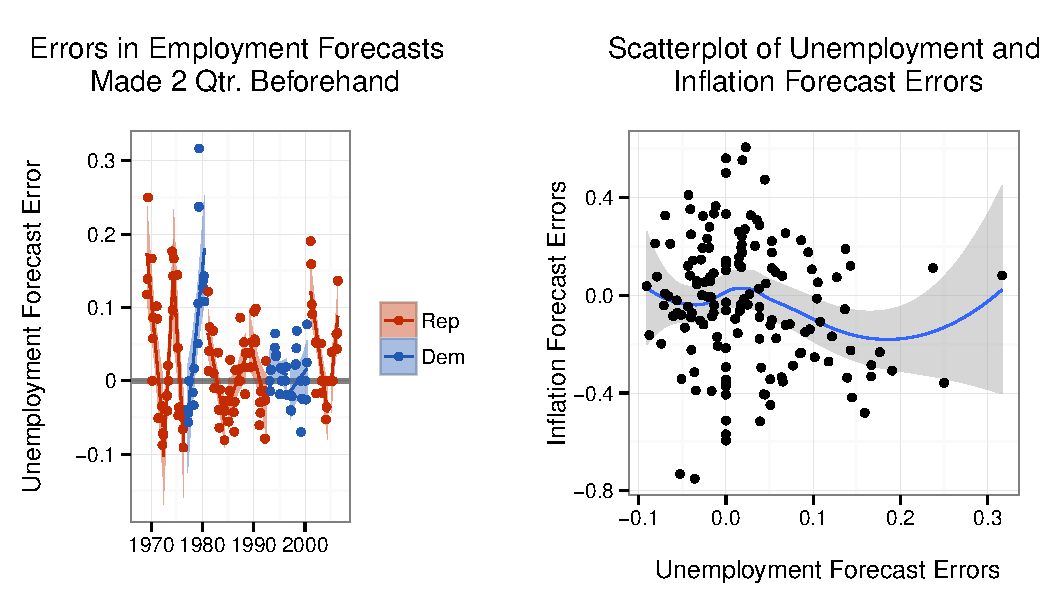
\includegraphics[width=0.95\linewidth]{figure/GraphPartisanErrorUnemploy} 

}



\end{knitrout}


    \end{center}
    \begin{singlespace}
        {\scriptsize{Note: Errors of 0 indicates that inflation/the unemployment rate was perfectly predicted.}}
    \end{singlespace}
\end{figure}

\subsection*{Matching to examine model dependence}

To further examine if our results depend on model specification, rather than an underlying causal effect, we follow recommendations from \cite{Ho2007} to pre-process the data using matching. This data is then used in our parametric regression models to estimate the relationships between our potential causal variables and Fed Staff inflation forecast errors. Doing this allows us to more robustly determine the effects of two `treatments' that Fed Staffers are exposed to that we are interested in: a partisan treatment and an electoral treatment. 

Pre-analysis matching allows us to mimic the conditions of a randomized experiment. Imagine an ideal world where we could create a controlled experiment to examine the causal relationship between, for example, presidential partisan ID and inflation forecast errors. Following the Neyman-Rubin causal model \citep{Sekhon2008} estimating causal effects is a comparison between potential outcomes for a hypothetical unit \citep{Stuart2010}. In our study the `unit' is a quarter being forecasted for. The casual effect of presidential party ID on inflation errors is a comparison of the inflation error for the particular quarter when the president is a Democrat and a Republican. We could approach this comparison in an experiment by randomly assigning presidents to quarters. In the language of experimental design the `treatment' could be a Democratic president and the `control' a Republican president. Note: in our analysis the determinations of `treatment' and `control' groups is arbitrary. This allows us to have groups of quarters that are as similar as possible except for the president's party ID. 

This is clearly impossible for us. Given that we are working with observational data, other variables that have an impact on forecast errors may have {\emph{different distributions}} across the treatment and control groups \citep{Cochran1973, Diamond2012}. It can be difficult to identify the relationships between presidential party ID, elections and errors from all of the confounding background variables.

Thus far we have attempted to address this issue statistically with models that allow us to estimate the effect of presidential party ID and elections on forecast errors `controlling for' a wide variety of other factors. However, it may be the case that our results are dependent on the model specifications \citep{Ho2007}. To examine this possibility we aimed to further recreate randomized experimental conditions with pre-analysis matching. We use the {\tt{R}} package {\tt{MatchIt}} \citep{matchit2011} to create two matched data sets where the non-treatment covariates in the control groups closely match those in the treatment groups.

Formally, each quarter $q$ in the data set is `assigned' to either the treatment group ($t_{q} = 1$) or the control group ($t_{q} = 0$). $y_{q}(1)$ is the potential outcome--in our case the inflation forecast error--for quarter $q$ of being in the treatment group, regardless of whether or not it was observed to be in this group. $y_{q}(0)$ is the potential outcome if $q$ was not in the treatment group, regardless of its observed assignment. It is impossible to observe both $y_{q}(1)$ and $y_{q}(0)$ at the same time. Instead we observe one version of $y_{q}=t_{q}y_{q}(1)-(1-t_{q})y_q(0)$. For each $q$ there is a fixed vector of exogenous confounders $X_{q}$. Ideally $t_{q}$ and $X_{q}$ are independent. However, this is not necessarily the case. The point of matching is to reduce or eliminate the relationship between $t_{q}$  and $X_{q}$ by selecting, dropping, and/or duplicating data. Ideally this process matches one treated quarter with one controlled quarter that has the same values of $X_{q}$, i.e. the distribution of covariates is the same in the treated and control groups \citep{matchit2011}. This is known as ``covariate balance" \cite[1]{Diamond2012}. Using matching to balance a data set ``break[s] the link between the treatment variables and the pre-treatment controls'', effectively replicating the conditions of a randomized experiment with observational data \cite[][2--3]{matchit2011}. 

Balance is usually achieved in matching with propensity scores: the probabilities that units were assigned the treatment given their covariates. The propensity score model is generally unknown \citep{Drake1993}. To find the propensity score model we use Diamond and Sekhon's \citeyearpar{Diamond2012} genetic matching method (GenMatch).\footnote{The method is implemented with {\tt{MatchIt}}. The original source code for our exact matching models can be found at {\url{http://bit.ly/OFdA4u}}.} GenMatch is a multivariate method that uses an evolutionary search algorithm to automate the search for the propensity score model that creates maximum balance. This minimizes the difficulty of ``manually and iteratively checking the propensity score" to determine covariate balance \citep[][2]{Diamond2012}. 

Once we created the matched data sets we then used them in in parametric models similar to those above. See results in tables \ref{OutputEL}, \ref{OutputPL},and \ref{OutputPB}. 

Before discussing the results, let's consider diagnostic tests we ran on the matching models. We primarily diagnosed the matching models with propensity score distribution plots--the probability of a quarter being in the `treated' group given its covariates--as well as quantile-quantile plots to diagnose whether or not each covariate in the matched data sets is balanced \citep{Ho2007}. Please see figures \ref{ElectPropensityScores} and \ref{PresPropensityScores} for the propensity score distributions in our matched data sets. The quantile-quantile plots are not shown, but can easily be created by running the original matching models in our main analysis source code file. The file is available at: \url{http://bit.ly/OFdA4u}. We are unable to achieve covariate balance for the Congressional interaction terms\footnote{The presidential party ID and election period interaction does balance.} and the Federal Reserve Chair variable. Chairs in our data set in the pre-Volcker/Greenspan era as well as current Chair Ben Bernanke were in office for very few observed quarters, making it difficult to match them. As such, we were not able to test the robustness of our findings for these variables with matched data.

Overall the results are similar when we use matched and non-matched data. Standard errors are larger in models using matched data than unmatched data. See Figure \ref{CoefComparePlots2} for the implications of the larger standard errors. Larger variance is likely because the sample sizes with matched data is smaller. For more details see: \url{http://bit.ly/U6edHt}. 

Notably both the point estimates and the uncertainty surrounding our key presidential partisan ID variable are very similar using both matched and non-matched data. We also did not find evidence that inflation forecast errors were associated with elections either independent of presidential party ID or in interaction with it in the matched models, including when we matched based on election period. This provides more evidence that our results are robustly estimating an actual causal effect and are not model dependent. 

%%%%%%% Table of  matched data with Normal Linear parametric model %%%%%%%%

\begin{table}[ht]
    \caption{Normal Linear Regression Estimation of Covariate Effects on 2 Qtr. Inflation Forecast Error (Matched by Election Period Variable)}
    \label{OutputEL}
    \vspace{0.25cm}
    \begin{center}
    {\tiny
 
\begin{tabular}{ l D{.}{.}{1}D{.}{.}{1}D{.}{.}{1}D{.}{.}{1}D{.}{.}{1}D{.}{.}{1}D{.}{.}{1}D{.}{.}{1}D{.}{.}{1}D{.}{.}{1}D{.}{.}{1}D{.}{.}{1}D{.}{.}{1} } 
\hline 
  & \multicolumn{ 1 }{ c }{ B1 } & \multicolumn{ 1 }{ c }{ B2 } & \multicolumn{ 1 }{ c }{ B3 } & \multicolumn{ 1 }{ c }{ B4 } & \multicolumn{ 1 }{ c }{ B5 } & \multicolumn{ 1 }{ c }{ B6 } & \multicolumn{ 1 }{ c }{ B7 } & \multicolumn{ 1 }{ c }{ B8 } & \multicolumn{ 1 }{ c }{ B9 } & \multicolumn{ 1 }{ c }{ B10 } & \multicolumn{ 1 }{ c }{ B11 } & \multicolumn{ 1 }{ c }{ B12 } & \multicolumn{ 1 }{ c }{ B13 } \\ \hline
 %                    & B1              & B2              & B3              & B4              & B5              & B6              & B7              & B8              & B9              & B10             & B11             & B12             & B13            \\ 
Intercept            & -0.8            & -0.7            & -0.8            & 5.8 ^\dagger   & 9.1 ^*          & 3.3             & -2.1            & -2.1            & -4.7            & 0.2             & -0.9            & -0.4            & -2.4 ^{***}    \\ 
                     & (4.0)           & (4.0)           & (4.0)           & (3.3)           & (4.0)           & (3.7)           & (4.1)           & (4.1)           & (4.7)           & (3.6)           & (3.7)           & (3.4)           & (0.7)          \\ 
Expenditure/GDP      & 0.2 ^{***}      & 0.2 ^{***}      & 0.2 ^{***}      & 0.2 ^{***}      &                 & 0.2 ^{***}      & 0.2 ^{***}      & 0.2 ^{***}      & 0.2 ^{***}      & 0.2 ^{***}      & 0.2 ^{***}      & 0.1 ^{***}      &                \\ 
                     & (0.0)           & (0.0)           & (0.0)           & (0.0)           &                 & (0.0)           & (0.0)           & (0.0)           & (0.0)           & (0.0)           & (0.0)           & (0.0)           &                \\ 
Output Gap           & -0.0            & -0.0            & -0.0            & -0.1 ^{**}      & -0.1 ^*         & -0.1 ^\dagger  & -0.0            & -0.0            & 0.0             & -0.0            & -0.0            & -0.1            &                \\ 
                     & (0.0)           & (0.0)           & (0.0)           & (0.0)           & (0.0)           & (0.0)           & (0.0)           & (0.0)           & (0.1)           & (0.0)           & (0.0)           & (0.0)           &                \\ 
Discount Rate Change & -0.0            & 0.0             & -0.0            & -0.1            & -0.5 ^*         & -0.1            & -0.2            & -0.2            & -0.3            & 0.1             & 0.1             & 0.3             &                \\ 
                     & (0.2)           & (0.3)           & (0.3)           & (0.2)           & (0.2)           & (0.2)           & (0.2)           & (0.2)           & (0.2)           & (0.2)           & (0.2)           & (0.2)           &                \\ 
Unemployment Rate    & -0.1            & -0.0            & -0.1            & 0.1             & 0.1             & 0.0             & -0.1            & -0.1            & -0.2 ^\dagger  & -0.1            & -0.1            & 0.0             &                \\ 
                     & (0.1)           & (0.1)           & (0.1)           & (0.1)           & (0.1)           & (0.1)           & (0.1)           & (0.1)           & (0.1)           & (0.1)           & (0.1)           & (0.1)           &                \\ 
Qtr. to Election     &                 & 0.0             &                 &                 &                 & 0.0             & 0.0             & 0.0             & -0.0            & 0.0             & 0.0             & 0.0 ^{**}       &                \\ 
                     &                 & (0.0)           &                 &                 &                 & (0.0)           & (0.0)           & (0.0)           & (0.0)           & (0.0)           & (0.0)           & (0.0)           &                \\ 
Qrt. to Election2    &                 & -0.0            &                 &                 &                 &                 &                 &                 & 0.0             &                 &                 &                 &                \\ 
                     &                 & (0.0)           &                 &                 &                 &                 &                 &                 & (0.0)           &                 &                 &                 &                \\ 
Election Period      &                 &                 & -0.0            &                 &                 &                 &                 &                 &                 &                 &                 &                 &                \\ 
                     &                 &                 & (0.1)           &                 &                 &                 &                 &                 &                 &                 &                 &                 &                \\ 
Pres. Party ID       &                 &                 &                 & 0.4 ^{***}      & 0.5 ^{***}      & 0.4 ^{***}      & 0.3 ^{***}      & 0.3 ^{***}      & 0.2             & 1.1 ^{***}      & 1.3 ^{***}      & 11.4 ^{***}     & 6.4 ^*         \\ 
                     &                 &                 &                 & (0.1)           & (0.1)           & (0.1)           & (0.1)           & (0.1)           & (0.1)           & (0.2)           & (0.3)           & (2.7)           & (2.8)          \\ 
Deficit/GDP          &                 &                 &                 &                 & -0.1 ^*         &                 &                 &                 &                 &                 &                 &                 &                \\ 
                     &                 &                 &                 &                 & (0.0)           &                 &                 &                 &                 &                 &                 &                 &                \\ 
FRB/GlobalModel      &                 &                 &                 &                 &                 & 0.1             &                 &                 & 0.0             &                 &                 &                 &                \\ 
                     &                 &                 &                 &                 &                 & (0.1)           &                 &                 & (0.2)           &                 &                 &                 &                \\ 
Senate Dem/Rep       &                 &                 &                 &                 &                 &                 & -0.5 ^*         & -0.5 ^*         & -0.6 ^*         & -0.3            & -0.2            & 1.4 ^\dagger   & 1.1 ^\dagger  \\ 
                     &                 &                 &                 &                 &                 &                 & (0.2)           & (0.2)           & (0.2)           & (0.2)           & (0.2)           & (0.8)           & (0.7)          \\ 
House Dem/Rep        &                 &                 &                 &                 &                 &                 & 0.7 ^{**}       & 0.7 ^{**}       & 0.7 ^*          & 0.7 ^{**}       & 0.6 ^{**}       & 1.6 ^{***}      & 2.1 ^{***}     \\ 
                     &                 &                 &                 &                 &                 &                 & (0.2)           & (0.2)           & (0.3)           & (0.2)           & (0.2)           & (0.4)           & (0.4)          \\ 
Pres*Qrt. Election   &                 &                 &                 &                 &                 &                 &                 &                 & 0.1             &                 &                 &                 &                \\ 
                     &                 &                 &                 &                 &                 &                 &                 &                 & (0.1)           &                 &                 &                 &                \\ 
Pres*Qrt. Election2  &                 &                 &                 &                 &                 &                 &                 &                 & -0.0            &                 &                 &                 &                \\ 
                     &                 &                 &                 &                 &                 &                 &                 &                 & (0.0)           &                 &                 &                 &                \\ 
Pres*House           &                 &                 &                 &                 &                 &                 &                 &                 &                 & -0.6 ^{***}     &                 & -11.6 ^{***}    & -8.1 ^*        \\ 
                     &                 &                 &                 &                 &                 &                 &                 &                 &                 & (0.1)           &                 & (2.7)           & (3.0)          \\ 
Pres*Senate          &                 &                 &                 &                 &                 &                 &                 &                 &                 &                 & -0.8 ^{***}     & -7.0 ^{**}      & -2.0           \\ 
                     &                 &                 &                 &                 &                 &                 &                 &                 &                 &                 & (0.2)           & (2.2)           & (2.1)          \\ 
House*Senate         &                 &                 &                 &                 &                 &                 &                 &                 &                 &                 &                 & -0.9 ^*         & -1.1 ^{**}     \\ 
                     &                 &                 &                 &                 &                 &                 &                 &                 &                 &                 &                 & (0.4)           & (0.4)          \\ 
Pres*House*Senate    &                 &                 &                 &                 &                 &                 &                 &                 &                 &                 &                 & 7.6 ^{***}      & 4.3 ^*         \\ 
                     &                 &                 &                 &                 &                 &                 &                 &                 &                 &                 &                 & (1.9)           & (2.1)           \\
 $N$                  & 61              & 61              & 61              & 61              & 61              & 61              & 61              & 61              & 61              & 61              & 61              & 61              & 61             \\ 
AIC                  & 17.7            & 21.5            & 19.5            & -10.1           & 12.2            & -8.5            & -14.2           & -14.2           & -9.3            & -30.4           & -27.2           & -44.0           & -20.4          \\ 
BIC                  & 59.9            & 80.6            & 70.2            & 40.6            & 62.9            & 59.1            & 61.7            & 61.7            & 100.5           & 54.0            & 57.2            & 65.7            & 47.1           \\ 
$\log L$            & 11.1            & 17.2            & 14.2            & 29.0            & 17.9            & 36.2            & 43.1            & 43.1            & 56.6            & 55.2            & 53.6            & 74.0            & 42.2            \\ \hline
 \multicolumn{14}{l}{\footnotesize{Standard errors in parentheses}}\\
\multicolumn{14}{l}{\footnotesize{$^\dagger$ significant at $p<.10$; $^* p<.05$; $^{**} p<.01$; $^{***} p<.001$}}\\
\multicolumn{14}{l}{\footnotesize{The recession variable is omitted because there was almost no variation in the matched data set.}}\\
\multicolumn{14}{l}{\footnotesize{The reason that there was no variation is because there were only two quarters with both a recession}}\\
\multicolumn{14}{l}{\footnotesize{and an election period in our data set.}} 
\end{tabular} 


    }
    \end{center}
\end{table}

%%%%%%% Table of pres_party matched data with Normal Linear Regression parametric model %%%%%%%%

\begin{table}[ht]
    \caption{Normal Linear Regression Estimation of Covariate Effects on 2 Qtr. Inflation Forecast Error (Matched by President's Party ID variable)}
    \label{OutputPL}
    \vspace{0.25cm}
    \begin{center}
    {\tiny
 
\begin{tabular}{ l D{.}{.}{1}D{.}{.}{1}D{.}{.}{1}D{.}{.}{1}D{.}{.}{1}D{.}{.}{1}D{.}{.}{1}D{.}{.}{1}D{.}{.}{1}D{.}{.}{1}D{.}{.}{1}D{.}{.}{1}D{.}{.}{1} } 
\hline 
  & \multicolumn{ 1 }{ c }{ C1 } & \multicolumn{ 1 }{ c }{ C2 } & \multicolumn{ 1 }{ c }{ C3 } & \multicolumn{ 1 }{ c }{ C4 } & \multicolumn{ 1 }{ c }{ C5 } & \multicolumn{ 1 }{ c }{ C6 } & \multicolumn{ 1 }{ c }{ C7 } & \multicolumn{ 1 }{ c }{ C8 } & \multicolumn{ 1 }{ c }{ C9 } & \multicolumn{ 1 }{ c }{ C10 } & \multicolumn{ 1 }{ c }{ C11 } & \multicolumn{ 1 }{ c }{ C12 } & \multicolumn{ 1 }{ c }{ C13 } \\ \hline
 %                    & C1              & C2              & C3              & C4              & C5              & C6              & C7              & C8              & C9              & C10             & C11             & C12             & C13            \\ 
Intercept            & 2.2             & 1.7             & 2.1             & 2.6             & -2.5            & 2.2             & -5.2            & -5.2            & -6.4            & -4.2            & -5.2            & -2.0            & 1.9            \\ 
                     & (4.2)           & (4.3)           & (4.2)           & (3.5)           & (3.5)           & (3.6)           & (4.3)           & (4.3)           & (4.9)           & (4.0)           & (4.1)           & (4.3)           & (1.8)          \\ 
Recession            & 0.2             & 0.2             & 0.2             & 0.1             & 0.0             & 0.2             & 0.1             & 0.1             & 0.1             & 0.2             & 0.1             & 0.2             &                \\ 
                     & (0.2)           & (0.2)           & (0.2)           & (0.2)           & (0.2)           & (0.2)           & (0.2)           & (0.2)           & (0.2)           & (0.1)           & (0.1)           & (0.2)           &                \\ 
Expenditure/GDP      & 0.1 ^*          & 0.1 ^*          & 0.1 ^*          & 0.2 ^{**}       &                 & 0.2 ^{**}       & 0.2 ^{***}      & 0.2 ^{***}      & 0.2 ^{***}      & 0.1 ^*          & 0.2 ^{**}       & 0.1             &                \\ 
                     & (0.1)           & (0.1)           & (0.1)           & (0.0)           &                 & (0.0)           & (0.1)           & (0.1)           & (0.1)           & (0.1)           & (0.0)           & (0.1)           &                \\ 
Output Gap           & -0.0            & -0.0            & -0.0            & -0.1            & 0.0             & -0.1            & 0.0             & 0.0             & 0.0             & 0.0             & 0.0             & 0.0             &                \\ 
                     & (0.1)           & (0.1)           & (0.1)           & (0.0)           & (0.0)           & (0.0)           & (0.0)           & (0.0)           & (0.1)           & (0.0)           & (0.0)           & (0.0)           &                \\ 
Discount Rate Change & -0.5            & -0.6 ^\dagger  & -0.6 ^\dagger  & -0.6 ^*         & -0.7 ^*         & -0.5 ^\dagger  & -0.5 ^\dagger  & -0.5 ^\dagger  & -0.5 ^\dagger  & -0.2            & -0.2            & -0.4            &                \\ 
                     & (0.3)           & (0.3)           & (0.3)           & (0.3)           & (0.3)           & (0.3)           & (0.2)           & (0.2)           & (0.3)           & (0.2)           & (0.3)           & (0.3)           &                \\ 
Unemployment Rate    & -0.0            & -0.0            & -0.0            & -0.0            & -0.1            & -0.0            & -0.2 ^*         & -0.2 ^*         & -0.2            & -0.1            & -0.1            & -0.2            &                \\ 
                     & (0.1)           & (0.1)           & (0.1)           & (0.0)           & (0.1)           & (0.1)           & (0.1)           & (0.1)           & (0.1)           & (0.1)           & (0.1)           & (0.1)           &                \\ 
Qtr. to Election     &                 & 0.0             &                 &                 &                 & 0.0             & 0.0             & 0.0             & 0.0             & 0.0             & 0.0             & 0.0             &                \\ 
                     &                 & (0.0)           &                 &                 &                 & (0.0)           & (0.0)           & (0.0)           & (0.1)           & (0.0)           & (0.0)           & (0.0)           &                \\ 
Qrt. to Election2    &                 & -0.0            &                 &                 &                 &                 &                 &                 & -0.0            &                 &                 &                 &                \\ 
                     &                 & (0.0)           &                 &                 &                 &                 &                 &                 & (0.0)           &                 &                 &                 &                \\ 
Election Period      &                 &                 & -0.1            &                 &                 &                 &                 &                 &                 &                 &                 &                 &                \\ 
                     &                 &                 & (0.1)           &                 &                 &                 &                 &                 &                 &                 &                 &                 &                \\ 
Pres. Party ID       &                 &                 &                 & 0.3 ^{***}      & 0.4 ^{***}      & 0.3 ^{***}      & 0.4 ^{***}      & 0.4 ^{***}      & 0.3             & 1.2 ^{***}      & 1.2 ^{**}       & -1.3            & -1.6           \\ 
                     &                 &                 &                 & (0.1)           & (0.1)           & (0.1)           & (0.1)           & (0.1)           & (0.3)           & (0.3)           & (0.4)           & (2.2)           & (1.9)          \\ 
Deficit/GDP          &                 &                 &                 &                 & -0.1            &                 &                 &                 &                 &                 &                 &                 &                \\ 
                     &                 &                 &                 &                 & (0.0)           &                 &                 &                 &                 &                 &                 &                 &                \\ 
FRB/GlobalModel      &                 &                 &                 &                 &                 & -0.1            &                 &                 & -0.1            &                 &                 &                 &                \\ 
                     &                 &                 &                 &                 &                 & (0.1)           &                 &                 & (0.1)           &                 &                 &                 &                \\ 
Senate Dem/Rep       &                 &                 &                 &                 &                 &                 & -1.3 ^{**}      & -1.3 ^{**}      & -1.1 ^*         & -0.8 ^*         & -0.7 ^\dagger  & -3.7            & -3.8 ^\dagger \\ 
                     &                 &                 &                 &                 &                 &                 & (0.4)           & (0.4)           & (0.4)           & (0.4)           & (0.4)           & (2.4)           & (2.0)          \\ 
House Dem/Rep        &                 &                 &                 &                 &                 &                 & 1.1 ^{**}       & 1.1 ^{**}       & 1.0 ^*          & 1.2 ^{***}      & 1.0 ^{**}       & -0.1            & -0.9           \\ 
                     &                 &                 &                 &                 &                 &                 & (0.3)           & (0.3)           & (0.4)           & (0.3)           & (0.3)           & (1.5)           & (1.4)          \\ 
Pres*Qrt. Election   &                 &                 &                 &                 &                 &                 &                 &                 & 0.0             &                 &                 &                 &                \\ 
                     &                 &                 &                 &                 &                 &                 &                 &                 & (0.1)           &                 &                 &                 &                \\ 
Pres*Qrt. Election2  &                 &                 &                 &                 &                 &                 &                 &                 & -0.0            &                 &                 &                 &                \\ 
                     &                 &                 &                 &                 &                 &                 &                 &                 & (0.0)           &                 &                 &                 &                \\ 
Pres*House           &                 &                 &                 &                 &                 &                 &                 &                 &                 & -0.7 ^*         &                 & -0.3            & 0.1            \\ 
                     &                 &                 &                 &                 &                 &                 &                 &                 &                 & (0.2)           &                 & (1.7)           & (1.6)          \\ 
Pres*Senate          &                 &                 &                 &                 &                 &                 &                 &                 &                 &                 & -0.8 ^*         & 4.1             & 4.5 ^*         \\ 
                     &                 &                 &                 &                 &                 &                 &                 &                 &                 &                 & (0.4)           & (2.9)           & (2.1)          \\ 
House*Senate         &                 &                 &                 &                 &                 &                 &                 &                 &                 &                 &                 & 1.8             & 2.3            \\ 
                     &                 &                 &                 &                 &                 &                 &                 &                 &                 &                 &                 & (1.7)           & (1.5)          \\ 
Pres*House*Senate    &                 &                 &                 &                 &                 &                 &                 &                 &                 &                 &                 & -1.7            & -2.2           \\ 
                     &                 &                 &                 &                 &                 &                 &                 &                 &                 &                 &                 & (1.8)           & (1.5)           \\
 $N$                  & 54              & 54              & 54              & 54              & 54              & 54              & 54              & 54              & 54              & 54              & 54              & 54              & 54             \\ 
AIC                  & 11.5            & 14.0            & 12.4            & -7.2            & 3.6             & -4.1            & -14.4           & -14.4           & -10.0           & -20.8           & -18.2           & -18.1           & -18.4          \\ 
BIC                  & 59.2            & 77.7            & 68.1            & 48.5            & 59.3            & 67.5            & 65.1            & 65.1            & 101.4           & 66.7            & 69.3            & 93.3            & 45.3           \\ 
$\log L$            & 18.3            & 25.0            & 21.8            & 31.6            & 26.2            & 38.1            & 47.2            & 47.2            & 61.0            & 54.4            & 53.1            & 65.0            & 41.2            \\ \hline
 \multicolumn{14}{l}{\footnotesize{Standard errors in parentheses}}\\
\multicolumn{14}{l}{\footnotesize{$^\dagger$ significant at $p<.10$; $^* p<.05$; $^{**} p<.01$; $^{***} p<.001$}} 
\end{tabular} 


    }
    \end{center}
\end{table}

%%%%%%% Table of pres_party matched data with Normal Bayesian linear parametric model %%%%%%%%

% latex table generated in R 3.0.2 by xtable 1.7-1 package
% Mon Nov 25 15:35:14 2013
\begin{table}[ht]
\centering
\caption{Bayesian Normal Linear Regression Estimation of Covariate Effects on 2 Qtr. Inflation Forecast Error (Matched by President's Party ID variable)} 
\label{OutputPB}
{\small
\begin{tabular}{lccccc}
  \hline
Variables & Mean & SD & 2.5\% & 50\% & 97.5\% \\ 
  \hline
Intercept & 2.17 & 3.64 & -4.84 & 2.15 & 9.57 \\ 
  Pres. Party ID & 0.33 & 0.07 & 0.19 & 0.33 & 0.48 \\ 
  Recession & 0.16 & 0.17 & -0.17 & 0.16 & 0.49 \\ 
  Qtr. to Election & 0.00 & 0.01 & -0.01 & 0.00 & 0.02 \\ 
  Expenditure/GDP & 0.16 & 0.05 & 0.06 & 0.16 & 0.25 \\ 
  Output Gap & -0.06 & 0.04 & -0.14 & -0.05 & 0.03 \\ 
  Discount Rate Change & -0.54 & 0.29 & -1.11 & -0.54 & 0.02 \\ 
  Unemployment Rate & -0.00 & 0.06 & -0.12 & -0.00 & 0.11 \\ 
  Global Model & -0.07 & 0.10 & -0.26 & -0.07 & 0.11 \\ 
  sigma2 & 0.05 & 0.01 & 0.03 & 0.05 & 0.07 \\ 
   \hline
\end{tabular}
}
\end{table}



%%%%%%% Matching Diagnostic Plots %%%%%%
%%%%% Elections %%%%%%%
\begin{figure}[h]
  \caption{Matched on Election Period}
  \label{ElectPropensityScores}
\begin{knitrout}
\definecolor{shadecolor}{rgb}{0.969, 0.969, 0.969}\color{fgcolor}

{\centering 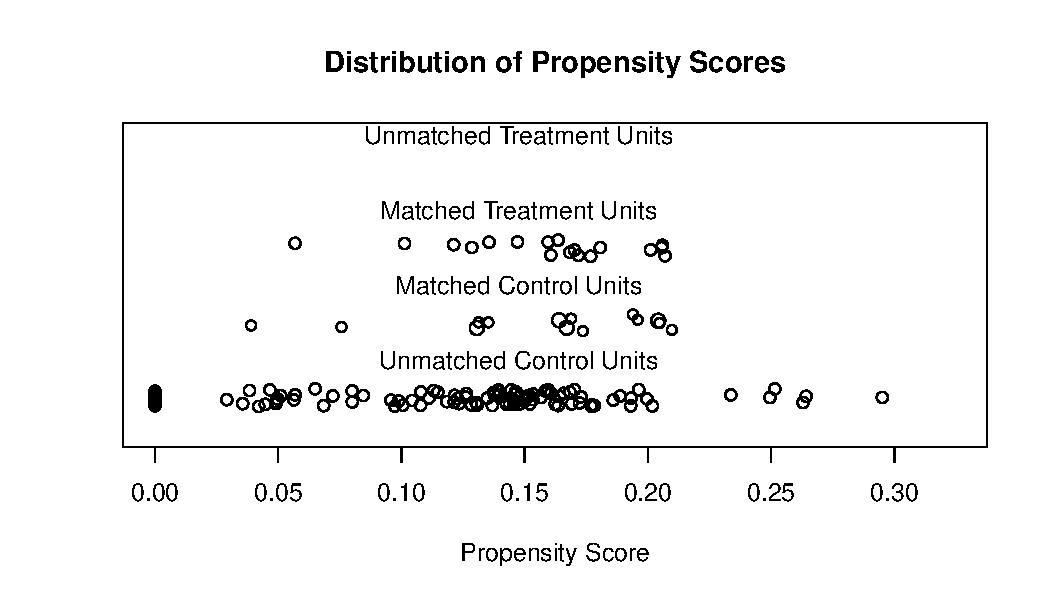
\includegraphics[width=\maxwidth]{figure/ElectPropensity} 

}



\end{knitrout}

    \begin{singlespace}
        {\scriptsize{Pre- and Post-matching propensity scores, where the ``Treated Units" are election quarters or the quarter before. ``Control Units" are from all other quarters. The more similar the distribution of matched treated and control unit propensity scores, the more successful the matching model was \cite[17]{Hollyer2012}.}}
    \end{singlespace}
\end{figure}

%%%%% Presidential Party ID %%%%%%
\begin{figure}[h]
  \caption{Matched on Presidential Party Identification}
  \label{PresPropensityScores}
\begin{knitrout}
\definecolor{shadecolor}{rgb}{0.969, 0.969, 0.969}\color{fgcolor}

{\centering 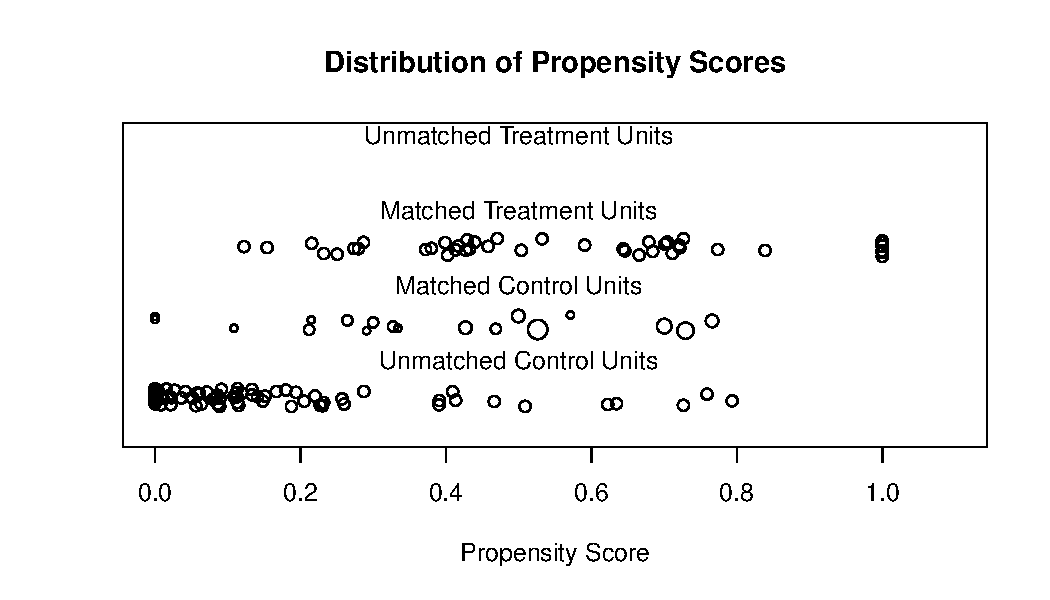
\includegraphics[width=\maxwidth]{figure/PresPropensity} 

}



\end{knitrout}

  \begin{singlespace}
      {\scriptsize{Pre- and Post-matching propensity scores, where the ``Treated Units" are quarters when the president was a Democrat. ``Control Units" are quarters when with a Republican president. The more similar the distributions of matched treated and control unit propensity scores, the more successful the matching model was \cite[17]{Hollyer2012}.}}
  \end{singlespace}
\end{figure}

\begin{figure}[t]
    \caption{95\% Confidence Bands for Coefficients from a Variety of Matching and Parametric Model Specifications}
    \label{CoefComparePlots2}
    \begin{center}

\begin{knitrout}
\definecolor{shadecolor}{rgb}{0.969, 0.969, 0.969}\color{fgcolor}

{\centering \includegraphics[width=0.95\linewidth]{figure/CoefComparePlotsMatched} 

}



\end{knitrout}

    \end{center}
    \begin{singlespace}
        {\scriptsize{Data matched by presidential party identification. Intercept values are not shown to maintain a reasonable scale for comparing covariate estimates.}}
    \end{singlespace}
\end{figure}

\subsection*{A brief history of inflation forecasting models at the US Federal Reserve (1970-2013)}

CASSIE CAN YOU FILL THIS IN? I THINK YOU CAN BASICALLY TAKE A LOT OF STUFF FROM WHAT YOU HAD WRITTEN BEFORE, BUT WE CUT FROM THE BODY OF THE TEXT.

EMPHASISE THAT EACH SHIFT IS PRETTY SMALL, JUSTIFYING THE FOCUS ON THE BIG SHIFT TO FRB GLOBAL.

\end{document}
